% Some notes:
%  1) Use Appel's SHA-256 implementation as an example
%

\documentclass[nocopyrightspace,preprint]{sigplanconf}

\usepackage[numbers]{natbib}

\usepackage[utf8]{inputenc} %for utf8 input
\usepackage{amssymb} %for shift symbol
\usepackage{amsmath}
\usepackage{listings} %for code
\usepackage{mathpartir} %for typing rules
\usepackage{microtype} %better micro typing
\usepackage{stmaryrd} %for llbracket
\usepackage{mathabx} % for boxes
\usepackage{graphicx} %to include png images
\usepackage{xcolor} %for colors
\usepackage{url}
\usepackage{enumitem}
\usepackage{array} %for stupid tables

%----------------------------------------------------

\usepackage{prettyref}
\newcommand{\pref}[1]{\prettyref{#1}}
\newcommand{\Pref}[1]{\prettyref{#1} \vpageref[]{#1}}
\newcommand{\ppref}[1]{\vpageref[]{#1}}
\newrefformat{fig}{Figure~\ref{#1}}
\newrefformat{app}{Appendix~\ref{#1}}
\newrefformat{tab}{Table~\ref{#1}}
\newrefformat{cha}{Challenge~\ref{#1}}
\newrefformat{compiler}{Point~\ref{#1} of \pref{thm:compiler}}

%----------------------------------------------------

\usepackage{amsthm}
\newtheorem{lemma}{Lemma}
\newtheorem{corollary}{Corollary}
\newtheorem{theorem}{Theorem}
\newtheorem{proposition}{Proposition}

%----------------------------------------------------

\lstset{
   numbers=none, %use numbers=left
   numberstyle=\tiny,
   stepnumber=1,
   numbersep=5pt,
   basicstyle=\tt\small,
   escapechar=\#,
   mathescape,
%   language=CaML,
   columns=flexible,
%   basewidth=0.455em,
   xleftmargin=\leftmargini,
%   xrightmargin=\leftmargini,
%   morekeywords={mod,div,matchD},
   deletekeywords={as},
   literate={<-}{$\;\leftarrow\;\;\,$}{3} {->}{$\;\rightarrow\;\;\,$}{3},
   firstnumber=auto % use name=NAME to identify split listings
%
% Placement: belowskip,aboveskip,lineskip,boxpos=l|c|r
%
% wonna figure-style listings? Use: caption={Useless code,label=useless
%
% keywordstyle=\color{black}\bfseries\underbar
% morekeywords={one,two,three,four}
}
% \lstinline!! 
% use basicstyle=\small ?

%How many languages are there in CompCert?
\newcommand{\howmanylanguages}[0]{11}

%How many passes are there in CompCert?
\newcommand{\howmanypasses}[0]{20}

\newcommand{\lines}[1]{\textsl{{\scriptsize #1}}}

\newcommand{\toolname}[0]{\ensuremath{C^4\!B} }

\newcommand{\valid}[6]{\ensuremath{\mathit{valid}(#1,#2,#3,#4,#5,#6)}}
\newcommand{\validC}[2]{\ensuremath{\mathit{validC}(#1,#2)}}
\newcommand{\safe}[4]{\ensuremath{\mathit{safe}(#1,#2,#3,#4)}}
\newcommand{\safeK}[5]{\ensuremath{\mathit{safeK}(#1,#2,#3,#4,#5)}}

\newcommand{\refines}[0]{\ensuremath{\prec}}

\newcommand{\qrefines}[0]{\ensuremath{\mathop{\prec_Q}}}

\newcommand{\pruned}[1]{\ensuremath{\overline{ #1} }}

\newcommand{\sem}[1]{\ensuremath{\llbracket #1 \rrbracket}}

\newcommand{\progs}[0]{\ensuremath{\mathcal{P}}}

\newcommand{\id}[0]{\ensuremath{\mathit{x}}}

\newcommand{\xevent}[0]{\ensuremath{\nu}}
\newcommand{\cevent}[0]{\ensuremath{\mu}}
\newcommand{\event}[0]{\ensuremath{\iota}}

\newcommand{\evalue}[0]{\ensuremath{v}}

\newcommand{\intval}[1]{\ensuremath{\mathsf{int}(#1)}}

\newcommand{\floatval}[1]{\ensuremath{\mathsf{float}(#1)}}

\newcommand{\call}[1]{\ensuremath{\mathsf{call}(#1)}}
\newcommand{\return}[1]{\ensuremath{\mathsf{ret}(#1)}}
\newcommand{\malloc}[1]{\ensuremath{\mathsf{malloc}(#1)}}
\newcommand{\free}[1]{\ensuremath{\mathsf{free}(#1)}}

\newcommand{\trace}[0]{\ensuremath{t}}

\newcommand{\Trace}[0]{\ensuremath{T}}

\newcommand{\conv}[2]{\ensuremath{\mathsf{conv}(#1,#2)}}

\newcommand{\divt}[1]{\ensuremath{\mathsf{div}(#1)}}

\newcommand{\fail}[1]{\ensuremath{\mathsf{fail}(#1)}}

\newcommand{\behav}[0]{\ensuremath{B}}

\newcommand{\getchar}[0]{\ensuremath{\mathsf{getchar}}}

\newcommand{\Z}[0]{\ensuremath{\mathbb{Z}}}
\newcommand{\N}[0]{\ensuremath{\mathbb{N}}}
\newcommand{\Qplusz}[0]{\ensuremath{\mathbb Q^+_0}}
\newcommand{\Q}[0]{\ensuremath{\mathbb{Q}}}

\newcommand{\weight}[2]{\ensuremath{W_{#2}(#1)}}
\newcommand{\tval}[2]{\ensuremath{V_{#2}(#1)}}

\newcommand{\prefs}[1]{\ensuremath{\mathit{prefs}(#1)}}

\newcommand{\type}[1]{\ensuremath{\mathsf{#1}}}

\newcommand{\code}[1]{\ensuremath{\mathsf{#1}}}

\newcommand{\env}[0]{\ensuremath{\mathit{\theta}}}

\newcommand{\mem}[0]{\ensuremath{\mathit{H}}}

\newcommand{\Mem}[0]{\ensuremath{\mathit{Mem}}}

\newcommand{\Var}[0]{\ensuremath{\mathit{Var}}}

\newcommand{\Val}[0]{\ensuremath{\mathit{Val}}}

\newcommand{\Aux}[0]{\ensuremath{\mathit{Aux}}}

\newcommand{\Input}[0]{\ensuremath{\mathit{StdIn}}}

\newcommand{\Assn}[0]{\ensuremath{\mathit{Assn}}}
\newcommand{\State}[0]{\ensuremath{\mathit{State}}}
\newcommand{\state}[0]{\ensuremath{\sigma}}

\newcommand{\Prop}[0]{\ensuremath{\mathit{Prop}}}

\newcommand{\ret}[0]{\ensuremath{\mathit{ret}}}

\newcommand{\htriple}[3]{\ensuremath{\{#1\}\, #2\, \{#3\}}}

\newcommand{\smallstep}[1]{\ensuremath{\to_{#1}}}

\newcommand{\conform}[2]{\ensuremath{\mathit{agree}(#1,#2)}}

\newcommand{\dom}[1]{\ensuremath{ \text{dom}(#1)}}
\newcommand{\img}[1]{\ensuremath{ \text{img}(#1)}}

\newcommand{\pimp}[2]{\ensuremath{#1 \Rightarrow #2}}

\newcommand{\Assert}[0]{\ensuremath{\mathit{Assert}}}

\newcommand{\VAssert}[0]{\ensuremath{\mathit{VAssert}}}

\newcommand{\eenv}[0]{\ensuremath{\Sigma}}

\newcommand{\genv}[0]{\ensuremath{\Delta}}

\newcommand{\fenv}[0]{\ensuremath{\Sigma}}

\newcommand{\Fundef}[0]{\ensuremath{\mathit{Fundef}}}

\newcommand{\funs}[0]{\ensuremath{\mathit{FID}}}

\newcommand{\vars}[0]{\ensuremath{\mathit{VID}}}

\newcommand{\statements}[0]{\ensuremath{\mathcal{S}}}

\newcommand{\traces}[0]{\ensuremath{\mathcal{T}}}

\newcommand{\behavs}[0]{\ensuremath{\mathcal{B}}}

\newcommand{\events}[0]{\ensuremath{\mathcal{E}}}

\newcommand{\initState}[2]{\ensuremath{\mathit{initSt}(#1,#2)}}

\newcommand{\retState}[1]{\ensuremath{\mathit{retState}(#1)}}

\newcommand{\Potential}[0]{\ensuremath{\mathit{Pot}}}

\newcommand{\evalE}[2]{\ensuremath{\llbracket #1 \rrbracket_{#2}}}

\newcommand{\Kseq}[2]{\ensuremath{\mathsf{Kseq}\, #1 \, #2}}

\newcommand{\Kloop}[2]{\ensuremath{\mathsf{Kloop}\, #1 \, #2}}

\newcommand{\Kstop}[0]{\ensuremath{\mathsf{Kstop}}}

\newcommand{\Kcall}[3]{\ensuremath{\mathsf{Kcall}\, #1 \, #2 \, #3}}

\newcommand{\cont}[0]{\ensuremath{K}}

\newcommand{\cost}[0]{\ensuremath{c}}

\newcommand{\used}[0]{\ensuremath{\sqbullet}}

\newcommand{\init}[0]{\ensuremath{\square}}

\newcommand{\FV}[1]{\ensuremath{\text{FV}(#1)}}

\newcommand{\loc}[0]{\ensuremath{\text{Loc}}}

\newcommand{\inter}[2]{\ensuremath{[#1,#2]}}

\newcommand{\ind}[0]{\ensuremath{\mathcal{I}}}

\newcommand{\states}[0]{\ensuremath{\mathcal{H}}}

\newcommand{\shift}[0]{{\lhd}}

\newcommand{\Vret}[0]{{\ensuremath{\mathit{ret}}}}
\newcommand{\Vargs}[0]{{\ensuremath{\vec {\mathit{args}}}}}

\newcommand{\tr}[0]{\ensuremath{\mathcal T}}

%-------------------------------------------------------
%Type rules (mathpatir)

\newcommand{\Rule}[4][]{\ensuremath{\inferrule*[right={\!(#2)},#1]{#3}{#4}}}
\newcommand{\RuleToplabel}[4][]{\ensuremath{\inferrule[(#2)]{#3}{#4}}}
\newcommand{\RuleNolabel}[3][]{\ensuremath{\inferrule*[#1]{#2}{#3}}}

%-------------------------------------------------------


%%% Local Variables: 
%%% mode: latex
%%% TeX-master: "main"
%%% End: 


\begin{document}

\conferenceinfo{POPL} {January XX-XX, 2014, CITY, STATE, India.}
\copyrightyear{2014}
\copyrightdata{XXX-X-XXXX-XXXX-X/XX/XX}

%----------------------------------------------------


\titlebanner{Draft -- Do not distribute}        % These are ignored unless
\preprintfooter{Draft}   % 'preprint' option specified.

\title{Compositional Certified Resource Bounds}
% Certified Resource Bounds for C
% Compositional Certified Resource Bounds for C
% Compositional Quantitative Resource Analysis of C Programs
% Compositional Resource-Bound Certification for C Programs

\authorinfo
{Quentin Carbonneaux \and Jan Hoffmann \and Zhong Shao}
{Yale University}


\maketitle


\begin{abstract}
  The goal of quantitative resource analysis is to provide developers
  with quantitative information about the runtime behavior of software
  at development time.  Recent years have seen tremendous progress in
  automatically deriving worst-case resource bounds.  Yet, many
  challenges in specifying, interactively deriving, formally
  certifying, and composing resource bounds remain unsolved.

  This paper describes a novel quantitative resource analysis
  framework that tackles these challenges for C programs.  The
  analysis framework consists of three parts.  First, the runtime
  resource consumption of programs is formalized with a parametric
  cost semantics for CompCert Clight.  Second, a quantitative Hoare
  logic that can be used for interactive bound development is
  implement and proved sound with respect to the cost semantics in the
  Coq Proof Assistant.  The logic is very expressive and shallow
  embedding enables a derived bound to be any function that is
  definable in Coq.  Third, an automatic amortized resource analysis
  for C programs that computes derivations in the quantitative Hoare
  logic is developed and implemented.  It is the first automatic
  amortized analysis that can derive bounds that depend on negative
  integers or differences between numbers, which is crucial to handle
  typical systems code.  Both, the quantitative logic and the
  automatic amortized analysis are naturally compositional and can be
  combined to semi-automatically derive global resource bounds.

  An experimental evaluation demonstrates the practicability of the
  analysis framework.  The expressivity of the logic is shown by
  manually deriving customized bounds that are tailored to specific
  algorithms.  A comparison of the automatic amortized analysis with
  other automatic tools on 30 challenging examples from the literature
  and open-source software shows that the bounds derived by the
  automatic amortized analysis are often more precise.
\end{abstract}

\category{D.2.4}{Software Engineering}
{Software/Program Verification}
\category{F.3.1}{Logics and Meanings of Programs}
{Specifying and Verifying and Reasoning about Programs}

\terms Verification, Reliability


\keywords Formal Verification, Compiler Construction, Program Logics,
Stack-Space Bounds, Quantitative Verification

\section{Introduction}
\label{sec:intro}

In software engineering and software verification, we often would like
to have static information about the quantitative behavior of
programs.  For example, stack and heap-space bounds are important to
ensure the reliability of safety-critical systems~\cite{veristack14,Regehr05}.
% Clock-cycle bounds are needed to guarantee the safety of real-time
% systems [XXX wilhelm].  
Static energy usage information is critical for autonomous systems and
has applications in cloud computing~\cite{CohenZSL12,CarrollH10}.
Worst-case time bounds can help to create constant-time
implementations that prevent side-channel
attacks~\cite{KasperS09,BartheBCLP14}.  Loop and recursion-depth
bounds are used to ensure the accuracy of programs that are executed
on unreliable hardware~\cite{CarbinMR13} and complexity bounds are
needed to verify cryptographic protocols~\cite{BartheGB09}.
% XXX Mention differential privacy here?
%
In general, quantitative performance information at design time can
provide useful feedback for developers.

Static analysis of quantitative properties of imperative programs is
an active research area and recent years have seen many innovations.
Notable tools that have been developed include
SPEED~\cite{GulwaniMC09}, KoAT~\cite{BrockschmidtEFFG14},
PUBS~\cite{AlbertAGPZ12}, Rank~\cite{AliasDFG10}, and LOOPUS~\cite{SinnZV14}.
%
While the these tools can derive impressive results for realistic
software, there still exist shortcomings that hamper the application
of the existing techniques in practice.
\begin{itemize}
\item Analysis tools are black boxes that either deliver a result or fail
  without enabling \emph{user interaction} to manually or
  semi-automatically derive bounds for challenging parts of the
  program.
\item The computed bounds are often \emph{non-compositional} local
  bounds (for a single (nested) loop) that are difficult to combine to
  global whole program bounds.
\item Existing techniques often rely on complex external tools such as
  abstract interpretation based invariant
  generation~\cite{GulwaniMC09} or translation of the program into a
  term-rewriting system~\cite{BrockschmidtEFFG14, SinnZV14} without
  providing \emph{verifiable certificates} for the correctness of the
  derived bound.
\end{itemize}
%
While there has been much progress in static quantitative analysis,
Knuth correctly points out in a recent interview~\cite{KnuthInter}
that the state-of-the-art in formal quantitative methods still falls
short in comparison with semantic techniques.
%
\begin{quote}
  % Consider, for example, a computer program that sorts a list of
  % numbers into order. 
  $[\cdots]$ Thanks to the work of Floyd, Hoare, and others,
  we have formal definitions of semantics, and tools by which we can
  verify that sorting is indeed always achieved. My job is to go
  beyond correctness, to an analysis of such things as the program's
  running time $[\cdots]$. I'm 100\% sure that my recurrence correctly
  describes the program's performance, and all of my colleagues agree
  with me that the recurrence is "obviously" valid. Yet I have no
  formal tools by which I can prove that my recurrence is right. I
  don't really understand my reasoning processes at all!
  \vspace{-3ex}
  \begin{flushright}
    -- Donald E. Knuth, 2014
  \end{flushright}
\end{quote}
%
In this work, we develop a resource analysis framework for C programs
that is based on a solid semantic foundation.  The choice of C is
primarily motivated by our ongoing work on the formally verified
hypervisor kernel CertiKOS~\cite{GuVFSC11}.  CertiKOS is mainly
developed in C and is supposed to provide verified guaranties on
timing and memory usage.  Moreover, C is a natural choice because it
is still the most widely used language for system development; in
particular in safety-critical embedded and real-time systems where
resource bound analyses are often required by regulatory
authorities~\cite{May2013}.  Our \emph{contributions} are as follows.
%
\begin{enumerate}
\item We define a operational cost semantics for CompCert Clight that
  defines the resource consumption of terminating and diverging
  executions.  The cost is parametric in a user-definable cost metric
  and can be negative if resources are released during an execution.
\item We develop a quantitative Hoare logic for interactively deriving
  resource bounds for Clight programs.  The logic is implemented and
  proved sound in the Coq Proof Assistant with respect to the cost
  semantics of Clight.
\item We describe an automatic static analysis that computes bounds
  together with derivations in the quantitative Hoare logic.  The
  analysis is inspired by type-based amortized resource analysis for
  functional programs~\cite{Jost03,HoffmannAH11}.  It computes
  derivations by generating simple linear constraints that can be
  solved by an off-the-shelf LP solver and does not require any
  fixpoint computations to obtain loop invariants.
\item We show with a publically available prototype implementation and
  an experimental evaluation that our novel amortized resource
  analysis works precisely and efficiently for common loop and
  recursion patterns, and that the derived constant factors in the
  bounds are close to or identical with the optimal ones.
% \item We prove the completeness of the program logic
%   with respect to the operational cost semantics.
\end{enumerate}
%
Our starting point is a recent work~\cite{veristack14} in which we
have formally verified bounds on the stack usage of C programs.  A key
part of this stack-bound verification is based on a quantitative Hoare
logic for deriving abstract stack bounds for CompCert Clight programs
that depend on the depth of (recursive) function calls.  % For
% non-recursive programs it is possible to compute derivations for such
% stack bounds in the quantitative Hoare logic automatically.  
By compiling these bounds together with the C program, we have derived
verified stack bounds for x86 assembly code.

Our \emph{first contribution} is a generalization of the quantitative
Hoare logic for CompCert Clight that enables us to derive resource
bounds that are parametric in the resource of interest.  The
quantitative logic is implemented in Coq and proved sound with respect
to a small-step operational cost semantics for Clight that counts a
constant resource consumption for each atomic execution step.  The
resource consumption at each step is parametric in a user-definable cost
metric and can be negative to express the release of resources (as
needed, e.g., to reason about memory usage).  Furthermore, a specific
\emph{tick} function can be inserted in the source code to further
customize the cost model.  In the implementation of the logic, we use
a shallow embedding in Coq which makes the logic very flexible.  There
is practically no limitation on the format of the derived resource
bounds since they can be any function that is definable in Coq.  The
derived bounds can also be parametric in a set of cost metrics or
specifically apply to one fixed cost metric.

The precision and expressivity of the quantitative Hoare logic provide
an ample foundation for reasoning about resource consumption of Clight
programs.  The logic is naturally compositional and the derived
\emph{quantitative Hoare triples} can be used to specify the resource
consumption of library functions or to describe resource contracts
between different functions.  However, reasoning about quantitative
properties can often be more tedious than reasoning about intentional
properties.  Consequently, automation is inevitable to derive resource
bounds for large code bases like CertiKOS.  Such an automation was
easily achievable in the case of constant stack bounds for a code base
that does not contain recursive functions~\cite{veristack14}.  In
general however, resource bounds have to be parametric in the
arguments of a function and depend on the number of loop iterations
and (recursive) function calls that are performed by the function.

For functional programs, there exist resource analysis systems---based
on type-based amortized resource analysis~\cite{Jost03,
  HoffmannAH12}---that can automatically derive complex polynomial
bounds with tight constant factors.  This type-based amortized
resource analysis has been our main inspiration in the design of the
quantitative Hoare logic and is therefore a natural candidate to
automate the reasoning.  However, it is a well-known problem that
type-based amortized resource analysis works well for functional
programs with pattern matching but not for C-like programs with
control flow that depends integer arithmetic.  For example, it is a
long-time open problem how to use type-based amortized analysis to
derive bounds for functions whose resource consumption depends on
(possibly negative) integers and non-sequential control flow as
introduced by \code{break} and \code{return} statements.
Unfortunately, these are the functions with non-constant resource
consumption that are most common in CertiKOS and other system
software.

Our \emph{second contribution} is an automatic amortized resource
analysis for CompCert Clight that computes derivations in the
quantitative Hoare logic.  It is the first automatic amortized
resource analysis that can derive bounds that depend on negative
integers and handles programs with mutually recursive functions as well as
\code{break} and \code{return} statements.  It targets programs that
are common in system software, that is, programs whose resource
consumption can be described as a function of sizes $|[x,y]| =
\max(0,y-x)$ of intervals of integer variables.  Such bounds arise for
instance from standard \emph{for loops} \code{for (i = x; i+K \leq y;
  i=i+K)} where the step-size $K>0$ is a constant.
%
The use of interval sizes in potential functions (an therefore in
resource bounds) is the main innovation that makes the analysis
practical for C.

Despite the apparent simplicity of the new analysis system, it is able
to reproduce results from the literature (e.g,
SPEED~\cite{GulwaniMC09}) that have been obtained using sophisticated
abstract-interpretation based methods.  In contrast with abstract-interpretation
based methods, our technique does not require any
fixpoint computations to obtain loop invariants.  The mechanism we
designed is able to leverage local assertions such as $x < y$ that we
collect along the branching points of the program to obtain global
resource invariants.  We achieve this by generating a linear
constraint system that reflects resource cost and size changes of
integer variables in the program.  A solution of the linear program
immediately yields a resource usage bound for the C
program.  % We can naturally, handle
% advanced control flow such as break, return, iteration over negative
% integer variables, and mutually-recursive functions.

Following the development steps of automatic amortized analysis for
functional programs~\cite{Jost03,HoffmannH10}, we deliberately
restrict ourselves to linear bounds in the automatic analysis (there
are no restrictions for the manually-derived bounds in the logic).
More specifically, bounds have the form $\sum_{a,b} q_{(a,b)} |[a,b]|$
where $a$ and $b$ are integer variables or constants.  The reason for
our focus on linear bounds is mainly clarity of presentation.  We
already experimented with an extension to multivariate resource
polynomials~\cite{HoffmannAH11,HoffmannS13} but this would make the inference
rules considerably more involved and should better be described
separately.  However, we developed the linear inference system so that
the extension to polynomial bounds shall work smoothly.

To the best of our knowledge, this article presents the first resource
analysis framework for C that makes it possible to combine non-trivial
automatically derived bounds with interactively derived bounds in a
proof system that produces verifiable certificates for the bounds.
Our approach complements existing work since it provides a semantic
foundation for the computation of bounds while still providing support
for automation that sometimes goes beyond the capabilities of existing
techniques.  Both the automatic amortized analysis and the
quantitative logic are naturally compositional and describe the
resource behavior of code fragments without referring to the source
code.  As a result, we naturally derive global bounds that are
functions of the input parameters of the program.  Another unique
feature of our system is, that it can handle resources like
memory that may become available during the execution.

We have evaluated the automatic analysis with system code and examples
from the literature.  \pref{app:cat} contains more than $30$
challenging loop and recursion patterns that we collected from open
source software and the literature.  Our analysis can find
asymptotically tight bounds for $30$ all but 3 of these patterns and
in most cases the derived constant factors are tight.  To compare our
automatic analyzer with existing techniques, we tested our examples
with the tools KoAT~\cite{BrockschmidtEFFG14},
PUBS~\cite{AlbertAGPZ12}, Rank~\cite{AliasDFG10}, and
LOOPUS~\cite{SinnZV14}.  We also contacted the authors of
SPEED~\cite{GulwaniMC09} but were able to obtain a tool to perform a
comparison.  Our experiments show that the bounds that we derive are
often more precise than those derived by existing tools.  Only
LOOPUS~\cite{SinnZV14}, which also uses amortization techniques, is
able to achieve a similar precision.

Several micro benchmarks demonstrate the practicability and
expressiveness of the quantitative Hoare logic.  For example, we
derive a logarithmic bound for a binary search function, a bound that
depends on the contents of an array to describe the exact cost of a
function that finds the maximal element in an array, and a linear
bound that amortizes the cost of $n$ successive increments to a binary
counter.  XXX In a larger case study, we show how the quantitative
logic can be used to derive the amortized cost for data-structure
operations for a table that expands or shrinks depending on the load
factor.

% To show the practicability of our approach we developed a case study
% with different real-time schedulers implemented in C.  To perform a
% schedulability analysis that takes into account the overhead of the
% scheduler we derived time bounds for context switching and
% initialization of the scheduler.  We then computed time bounds for a
% set of given user task and took account the previously computed
% scheduler overhead to determine whether the scheduling requirements of
% all user tasks can be met.

% With the intention, of making the material easily accessible we first
% informally describe the new automatic amortized analysis
% (\pref{sec:inform}).  We then formalize the intuition with the
% operational cost semantics an the inference rules for the amortized
% analysis (\pref{sec:aa}).  In \pref{sec:logic} we describe the
% quantitative Hoare logic and its soundness proof that is formalized in
% Coq.  In \pref{sec:inter} we prove the soundness of the automatic
% amortized analysis by showing that derivation using the inference
% rules can be seen as derivations in the quantitative logic.  We also
% show how to integrate hand-derived bounds with automatically-derived
% bounds.  \pref{sec:exper} contains the results of the experimental
% evaluation and \pref{sec:related} describes related research.


\section{Informal Account}
\label{sec:inform}

In this section, we informally introduce the quantitative program
logic and the automatic amortized analysis for for Clight programs.
The purpose of this section is to build some intuition that should
make the following sections, which contain more details, easy to read.

\subsection{Quantitative Hoare Logic}

The idea that drives the design of our system is amortized
analysis~\cite{Tarjan-amort}.  Assume that a program $S$
executes on a starting state $\state_0$ and consumes $n$ resource units
of some quantity we are interested in.  We denote that by writing $(S,
\state_0) \Downarrow_n$.  The basic idea of amortized analysis is to
define a potential function $\Phi$ that maps program states to
non-negative numbers and to show that $\Phi(\state) \geq n$ if
$\state$ is a program state such that such that $(S, \state)
\Downarrow_n$.

Since programs can be composed we must enrich the evaluation judgement
$(S, \state) \Downarrow_{n}$ to talk about the state resulting from
the program execution.  We write $(S, \state) \Downarrow_n \state'$ to
say that $\state'$ is the program state after the execution of $S$ in
starting state $\sigma$.  We now use two potential functions, one that
applies before the execution, and one that applies after.  The two
functions must respect the relation $\Phi(\state) \ge n +
\Phi'(\state')$ for all states $\state$ and $\state'$ such that $(S,
\state) \Downarrow_n \state'$.  Intuitively, $\Phi(\state)$ must
provide enough \emph{potential} for both, paying for resource cost of
the computation and paying for the potential $\Phi'(\state')$ on the
resulting state $\state'$. That way, if $(\state, S_1) \Downarrow_n
\state'$ and $(\state', S_2) \Downarrow_m \state''$, we get
$\Phi(\state) \ge n + \Phi'(\state')$ and $\Phi'(\state') \ge m +
\Phi''(\state'')$.  This can be composed to $\Phi(\state) \ge (n + m)
+ \Phi''(\state'')$.  Note that the initial potential function $\Phi$
provides an upper bound on the resource consumption of the whole
program.  What we have observed is that, if we define $\htriple{\Phi}
{S}{\Phi'}$ to mean
$$
\forall \state\, n\, \state'.\, (\state, p) \Downarrow_n \state' \implies \Phi(\state) \ge
n + \Phi'(\state')
$$
then we get the following familiar looking rule.
$$
\RuleNolabel
{\htriple{\Phi}{S_1}{\Phi'} \\ \htriple{\Phi'}{S_2}{\Phi''}}
{\htriple{\Phi} {S_1; S_2}  {\Phi''}}
$$
%
Similarly, other language constructs lead to rules for the potential
functions that look very similar to Hoare logic or effect systems
rules.  These rules enable interactive reasoning about resource usage
in a flexible and compositional way, which, as a side effect, produces
a certificate for the derived resource bound.

We have implemented and proved sound such a quantitative Hoare for
CompCert Clight in the Coq Proof Assistant.  Because we use a shallow
embedding in Coq, every function that can be expressed in Coq can in
principle be used as a resource bound.  We can use the logic to prove
a concrete bound for a given resource metric, or a bound that is
parametric in a set of resource metrics.  It is also possible to
incorporate boolean preconditions into the bounds to express that the
bound is only valid for a certain class of inputs.  To this end, we
allow the potential function $\Phi$ in the pre and post conditions to
take non-negative number or $\infty$ (infinity) as values.  Infinity,
plays the same role as $\mathit{false}$ in Hoare logic.  Boolean assertions can
be embedded into potential functions by mapping $\mathit{false}$ to $\infty$ and
$\mathit{true}$ to $0$.

\begin{figure}
\center
\begin{minipage}[b]{0.8\linewidth}
\begin{lstlisting}
${\color{blue}%
  \{ \#_1(a) + 2k \}}$
while (k > 0) {
  x=0;
  ${\color{blue}%
    \{ \#_1(a) + 2k \}}$
  while (x < N && a[x] == 1) {
    ${\color{blue}%
      \{ (a[x] = 1) + \#_1(a) + 2k \}}$
    a[x]=0;
    ${\color{blue}%
      \{ \#_1(a) + 2k + 1 \}}$
    tick(1);
    ${\color{blue}%
      \{ \#_1(a) + 2k \}}$
    x++; }
  ${\color{blue}%
    \{ (x \ge N \lor a[x] = 0) + \#_1(a) + 2k \}}$
  if (x < N) {
    ${\color{blue}%
      \{ (a[x] = 0) + \#_1(a) + 1 + 2(k-1) + 1 \}}$
    a[x]=1;
    ${\color{blue}%
      \{ \#_1(a) + 2(k-1) + 1 \}}$
    tick(1); }
  ${\color{blue}%
    \{ \#_1(a) + 2(k-1) \}}$
  k--;
  ${\color{blue}%
    \{ \#_1(a) + 2k \}}$
} ${\color{blue} \{ \#_1(a) \}}$

\end{lstlisting}
\end{minipage}

\caption{Example derivation using amortized reasoning.  We write
  $\#_1(a)$ for $\# \{ i \mid 0 \le i < N \land a[i] = 1 \}$ and use the
  tick metric that assigns cost $n$ to \lstinline{tick(n)} statements and
  0 to other operations.
  }
\label{fig:xmplinc}
\end{figure}




It is for instance possible to derive the following quantitative
triple for a binary-search that holds for all stack metrics $M$.  A
stack metric assigns cost $0$ to all evaluation steps except function
calls.  Before a call $f(x)$, we consume $M_f > 0$ resources and
after the call we return $M_f$ resources that can be used in
subsequent function calls.  So $M_f$ corresponds to the stack-frame
size of the function $f$.
%
\begin{center}
${ \{ (Z = \log_2(h-l)) + Z{\cdot}M_\code{bsearch} \} }$
\code{bsearch(x,l,h)}
${ \{ Z{\cdot}M_\code{bsearch} \} }$
  
\end{center}
%
In the pre and post condition, the logical variable $Z$ is used to
relate the size of the input with the potential that is left after the
function call.  The logical part $Z = \log_2(h-l)$ of the precondition
is $0$ if $Z = \log_2(\state_0(h)-\state_0(l))$ in the initial state
$\state_0$ and $\infty$ otherwise.

Assume for the remainder of this section that we are interested in
bounding the number of \emph{ticks} in a program.  In other words, we
use a resource metric that assigns cost $n$ to the function call
\code{tick(n)} and cost $0$ to all other operations.  The argument $n$
is an integer and a negative number means that $-n$ resources are
returned.

We say that the analysis is amortized because the use of a potential
function $\Phi$ enables us to amortize the cost of operations like in
typical textbook examples that use the potential method of Tarjan's
amortized analysis.  As an illustrative example, \pref{fig:xmplinc}
shows a program that repeatably increments a binary counter that is
implemented with a boolean-valued ($0$ or $1$) array.  The derived
bound in the precondition states that the number of ticks that are
executed by the program are bounded by $\#_1(a) + 2k$.  Here, $k$ is
the number of increments to the counter that are performed by the
program and $ \#_1(a) = \# \{ i \mid 0 \le i < N \land a[i] = 1 \}$ is
the number of $1$'s in the array $a$.  We have inserted the statement
\code{tick(1)} into the program whenever we update the array $a$.

To derive the bound for the program in~\pref{fig:xmplinc} in the
quantitative Hoare logic, we follow the textbook
reasoning~\cite{Algorithms}.  When we assign \code{a[x]=0} in the
inner loop, we know that $a[x]=1$ before the assignment.  As a result,
we have $\#_1(a) = \#_1(a') + 1$ if $a'$ is the array $a$ after the
assignment.  So we obtain one resource unit in addition to the
invariant (i.e., $\Phi = \#_1(a) + 2k + 1$) that we can use to pay for the
cost of the statement \code{tick(1)}.  To pay for the tick statement
in the conditional, we use the fact that $k>0$ to write $2k$ as $1 +
2(k-1) +1$.  Dual to the first assignment, we have $\#_1(a) +1 =
\#_1(a')$ if $a$ is the array before and $a'$ is the array after the
assignment \code{a[x]=1}.  After paying one potential unit for the
statement $\code{tick(1)}$, we are left with the potential $\#_1(a) +
2(k - 1)$.  But since we increment $k$ at the end of the outer loop,
we can establish again our loop invariant $\#_1(a) + 2k$.

See Section XXX for more a formal definition of the logic and
additional example derivation.

% For example we have the following judgement (provided that initially
% $\state_0(\code x) \ge \state_0(\code y) \ge 0$).
% $$
% \htriple
% {2{\cdot}x + 10}
% {\code{ x = x -  y}}
% {2{\cdot}x + 2{\cdot}y + 10}
% $$
% This must be understood as a motion of potential from the
% variable~$\code x$ to the variable~$\code y$. If some resource is
% consumed $\code y$ times afterwards, we can then use $\code y$'s
% potential to pay for it. However, the initial potential function
% $\Phi$ only refers to the variable~$\code x$: the potential function
% allows us to pass on the cost of the subsequent resource consumption
% to~$\code x$.  This flexibility combined with intelligent decisions on
% potential motions allows us to design an automatic analysis to
% discover linear invariants for surprisingly convoluted programs.



\subsection{Automatic Amortized Analysis}

A program logic provides a principled foundation for statically
analyzing programs.  However, program logics need to be supported by
automatic methods to be useful in practice.  That is why we developed a
new automatic amortized analysis for deriving quantitative Hoare
triples for common C programs.

To this end, we fix the shape of the potential functions $\Phi$ so
that it becomes possible to use \emph{linear programming} (LP) to
compute a derivation in the logic.  If we assume that a program state
$\state$ simply maps variable to integers then we require
$$
\Phi(\state) = q_0 + \sum_{x,y \in \dom{\state}} q_{(x,y)} {\cdot} |[\state(x),\state(y)]|
$$
where $q_{(x,y)} \in \Qplusz$ and $|[a,b]| = \max(b-a,0)$.  Note that
$q_0$ is the constant potential and that we treat constants as program
variables.  For instance, we always have $q_{(0,x)}|[0,x]|$ as a
component of $\Phi(\state)$ if $x \in \dom{\state}$.
%
We then develop an inference rule for each syntactic construct that
derives sound triples $\htriple{\Phi}P{\Phi'}$ in the quantitative
logic but enables inference by using an LP solver.  

This idea is best explained by example.  If we again use the
\emph{ticks} metric that assigns cost $n$ to the function call
\code{tick(n)} and cost $0$ to all other operations then the cost of
the following example can be bounded by $|[x,y]|$.
\begin{lstlisting}
while (x<y) {x=x+1; tick(1);} #\hfill \textnormal{(Example 1)}#
\end{lstlisting}
To derive this bound in our automatic amortized analysis, we start
with the initial potential $\Phi_0 = |[x,y]|$ (short for
$\Phi_0(\state) = |[\state(x),\state(y)]|$) which we also use as the
loop invariant.  For the loop body we then (like in Hoare logic) have
to derive a triple like
$\htriple{\Phi_0}{\code{x=x+1;tick(1)}}{\Phi_0}$.  However, we can
only do so if we utilize the fact that $x<y$ at the beginning of the
loop body.  The reasoning then works as follows.  We start with the
potential $|[x,y]|$ and the fact that $|[x,y]| > 0$ before the
assignment.  If we denote the updated version of $x$ after the
assignment by $x'$ then the relation $|[x,y]| = |[x',y]| + 1$ between
the potential before and after the assignment \code{x=x+1} holds.
This means that we have the potential $|[x,y]| + 1$ before the
statement \code{tick(1)}.  Since \code{tick(1)} consumes one resource unit,
we end up with potential $|[x,y]|$ after the loop body and have
established the loop invariant again.


\begin{figure}[t]
  \centering
\begin{lstlisting}[mathescape]
${\color{blue}%
  \cdot; \, 0 + \frac{T}{K} {\cdot} |[x,y]| + 0 {\cdot} |[y,x]| \vdash }$
while (x+K<=y) {
  ${\color{blue}%
  x + K \le y; \; 0 + \frac{T}{K} {\cdot} |[x,y]| + 0 {\cdot} |[y,x]| \vdash }$
  x=x+K; 
  ${\color{blue}%
  \dashv x \leq y; \, T + \frac{T}{K} {\cdot} |[x,y]| + 0 {\cdot} |[y,x]| \vdash }$
  tick(T);
  ${\color{blue}%
  \dashv x \leq y; \, 0 + \frac{T}{K} {\cdot} |[x,y]| + 0 {\cdot} |[y,x]| }$
}
${\color{blue}%
 \dashv x \geq y; 0 + \frac{T}{K} {\cdot} |[x,y]| + 0 {\cdot} |[y,x]|}$
\end{lstlisting}
  \caption{Automatic derivation of a tight bound on the number of
    ticks for a standard \emph{for loop}.  The parameters $K>0$ and
    $T>0$ are not program variables but denote a concrete constants in
    the program.  The reasoning works uniformly for all such $K$ and
    $T$.}
  \label{fig:ex1}
\end{figure}
More formally, we develop (in section XXX) a judgement 
$$
\Gamma; Q \vdash S \dashv Q'; \Gamma'
$$
such that $\Gamma$ contains logical assertions like $x<y$ that we
collect along the conditional branches of the program and $Q$ is a
family of coefficents $Q = (q_{(a,b)})_{a,b \in \text{scope}}$ that is
indexed by the variables that are currently in scope.  The logical
context $\Gamma$ is simply a conjunction of inequalities between
linear combinations variables.  It is used to determine at the
assignment if we can extract constant potential to pay for future
cost.  It is important to note that the reasoning about assertions in
$\Gamma$ are very basic.  We do not perform any fixpoint computations
and only derive trivial loop invariants about variables that are
unchanged in the loop body.

Note that our notion of a potential function is a refinement of the
concept of a ranking function.  A potential function can be used like
a ranking function if we use the tick metric and add the statement
\code{tick(1)} to every back edge of the program (loops and function
calls).  However, a potential function is more flexible.  For example,
we can use a potential function to prove that Example~2 does not
consume any resources in the tick metric.
\begin{lstlisting}
  while (x<y) {tick(-1); x=x+1; tick(1);} #\hfill \textnormal{(Example 2)}#
\end{lstlisting}
Similarly we can prove that Example~3 can be bounded by $10|[x,y]|$.
In both cases, we reason exactly like in the first version of the
while loop to prove the bound.  Of course, such loops with different
tick annotations can be seamlessly combined in a larger program.
\begin{lstlisting}
  while (x<y) {x=x+1; tick(10);} #\hfill \textnormal{(Example 3)}#
\end{lstlisting}
%
\pref{fig:ex1} shows a derivation of the bound
$\frac{T}{K}{\cdot}|[x,y]|$ on the number of ticks for a generalized
version of Example~1 in which increment $x$ be a constant $K>0$ and
consume $T>0$ resources in each iteration.  The reasoning is similar
to the description of Example~1 except that we obtain the potential
$K{\cdot}\frac{T}{K}$ after the assignment.  Note that the logical
assertions in $\Gamma$ are only used in rule for the assignment
\code{x=x+K}.  To the best of our knowledge, no other tool is
currently capable of deriving a tight bound on the cost of such a
loop.  For $T=1$ (many systems focus on the number of loop iterations
without a cost model) and $K=10$, KoAT~\cite{BrockschmidtEFFG14}
computes the bound $x + y + 10$, PUBS~\cite{AlbertAGPZ12} computes
the tight bound $0.1(y-x)$, Rank~\cite{AliasDFG10} computes the bound XXX, and
LOOPUS~\cite{SinnZV14} computes the bound $y-(x+9)$.

It might be surprising that we only track simple linear relations in
the logical context $\Gamma$.  It would of course be possible to keep
track more sophisticated assertions.  However, this simple form is
sufficient for the examples we considered and we can efficiently
decide queries such as $\Gamma \implies x<y \; ?$ that we make in the
assignment rule.  Nevertheless, this logical part of our analysis
system is orthogonal to the quantitative part and can be easily
extended if necessary.

To understand the capabilities of the automatic analysis, it is
instructive to study more involved examples.  \pref{fig:ex_list}
contains Examples \emph{speed\_1} and \emph{speed\_2} that are taken
from previous work on bound analysis~\cite{GulwaniMC09}.  The SPEED
tool~\cite{GulwaniMC09} derives the bounds as our analysis but
requires inference of a \emph{disjunctive invariant}.  In the abstract
interpretation community, these invariants are known to be notoriously
difficult to handle.
%
In example \emph{speed\_1} we have one loop that first increments
variable $y$ up to $m$ and then increments variable $x$ up to $n$.  We
derive the tight bound $|[x, n]| + |[y, m]|$.
%
Example \emph{speed\_2} is more tricky and trying to understand how it
works may be challenging.  However, with the amortized analysis in
mind, using the potential transfer reasoning, it is almost trivial to
prove a bound.  While the SPEED tool has to find a fairly
involved invariant for the loop, our tool is simply reasoning locally
and works without any clever tricks. We obtain the tight bound $|[x,
n]| + |[z, n]|$.

Example \emph{t08} shows the ability of the analysis to handle
negative and non-negative numbers.  Note that there are no
restrictions on the signs of $z$ and $y$.  We also see that we can
accurately track the size change of $y$ in the first loop.
Furthermore, \emph{t08} shows that we do not handle the constants $1$
or $0$ in any special way.  In all examples you could replace $0$ and
$1$ with other constants like we did in the second loop and still
derive a tight bound.  The only information, that the analyzer needs
is $y \geq c$ before assigning $y = y - c$.

Example \emph{t27} shows how amortization can be used to handle tricky
nested loops.  The outer loop we increment the variable $n$ till $n =
0$.  In each of the $|[n,0]|$ iterations, we increment the variable
$y$ by $1000$.  We then non-deterministically execute an inner loop
that decrements $y$ by $100$ until $y<100$.  The analysis can derive
that only the first execution of the inner loop depends on the initial
value of $y$.  We again derive tight constant factors.

As mentioned, the analysis naturally handles advanced control flow
like \code{break} and \code{return} statements, and mutual recursion.
\pref{fig:ex_rec} contains two mutually-recursive functions with their
automatically derived tick bounds.  The function \code{count\_down}
decrements its first argument $x$ until it reaches the second argument
$y$. It then recursively calls the function \code{count\_up}.  The
function \code{count\_up} is dual to \code{count\_down}.  Here, we
count up $y$ by $2$ and recursively call \code{count\_down}.  Our
analysis system can compute a tight bound.  On this example, the
analysis amounts to computing the meeting point of two trains that
approach each other with different speeds.
% This is comparable to the
% determination of the point at which to trains meet if they approach
% each other with different speeds.

We only show a very small selections of the programs that we can
handle automatically here.  In \pref{app:cat} you find a list of more
than $30$ classes of challenging programs that we can automatically
analyze.  We hope that this gives you an impression of the
capabilities of the analysis but we also point out that this list is
far from being exhaustive.

\newlength{\progwidth}

\begin{figure*}[t!]
 \setlength{\progwidth}{.22\linewidth}
  \centering
\hspace{-0.4cm}
  \begin{minipage}[b]{.18\linewidth}
    \begin{center}
   \begin{lstlisting}[]
while (n>x) {
  ${\color{blue}%
  n{>}x; \, |[x, n]| {+} |[y, m]| \vdash }$
  if (m>y) 
    ${\color{blue}%
    m{>}y; \, |[x, n]| {+} |[y, m]| \vdash }$
    y = y+1;
    ${\color{blue}%
    \dashv \cdot ; \, 1 {+} |[x, n]| {+} |[y, m]| }$
  else
    ${\color{blue}%
    n{>}x; \, |[x, n]| {+} |[y, m]| \vdash }$
    x = x+1;
    ${\color{blue}%
    \dashv \cdot; \, 1 {+} |[x, n]| {+} |[y, m]| }$
  ${\color{blue}%
  \dashv \cdot; \, 1 {+} |[x, n]| {+} |[y, m]| \vdash }$
  tick(1);
  ${\color{blue}%
  \dashv \cdot; \, |[x, n]| {+} |[y, m]| }$
}
   \end{lstlisting}

$|[x, n]| + |[y, m]|$
\\[.7\baselineskip]
      {\bf speed\_1}
    \end{center}
  \end{minipage}
%
\hfill
%
  \begin{minipage}[b]{\progwidth}
    \begin{center}
   \begin{lstlisting}

while (x<n) {
  ${\color{blue}%
  x{<}n; \, |[x, n]| {+} |[z, n]| \vdash }$
  if (z>x)
    ${\color{blue}%
    x{<}n; \, |[x, n]| {+} |[z, n]| \vdash }$
    x=x+1;
    ${\color{blue}%
    \dashv \cdot; \, 1 {+} |[x, n]| {+} |[z, n]| }$
  else
    ${\color{blue}%
    z{\leq}x, x{<}n; \, |[x, n]| {+} |[z, n]| \vdash }$
    z=z+1;
    ${\color{blue}%
    \dashv \cdot; \, 1 {+} |[x, n]| {+} |[z, n]| }$
  ${\color{blue}%
  \dashv \cdot; \, 1 {+} |[x, n]| {+} |[z, n]| \vdash }$
  tick(1);
  ${\color{blue}%
  \dashv \cdot; \, |[x, n]| {+} |[z, n]| }$
  }
   \end{lstlisting}

$|[x, n]| + |[z, n]|$
\\[.7\baselineskip]
      {\bf speed\_2}
    \end{center}
  \end{minipage}
%
\hfill
%
  \begin{minipage}[b]{\progwidth}
    \begin{center}
   \begin{lstlisting}
while (z-y>0) {
  ${\color{blue}%
  y{<}z; \, 3.1|[y,z]| {+} 0.1|[0,y]| \vdash }$
  y = y+1;
  ${\color{blue}%
  \dashv \cdot; \, 3 {+} 3.1|[y,z]| {+} 0.1|[0,y]| \vdash }$
  tick(3);
  ${\color{blue}%
  \dashv \cdot; \, 3.1|[y,z]| {+} 0.1|[0,y]| }$
}
${\color{blue}%
\dashv \cdot; \, 3.1|[y,z]| {+} 0.1|[0,y]| \vdash }$
while (y>9) {
  ${\color{blue}%
  y{>}9; \, 3.1|[y,z]| {+} 0.1|[0,y]| \vdash }$
  y=y-10;
  ${\color{blue}%
  \dashv \cdot; \, 1 {+} 3.1|[y,z]| {+} 0.1|[0,y]| \vdash }$
  tick(1);
  ${\color{blue}%
  \dashv \cdot; \, 3.1|[y,z]| {+} 0.1|[0,y]| }$
}
   \end{lstlisting}

$3.1|[y,z]| + 0.1|[0,y]|$
\\[.7\baselineskip] 
      {\bf t08}
    \end{center}
  \end{minipage}
%
\hfill
%
%
%
  \begin{minipage}[b]{\progwidth}
    \begin{center}
   \begin{lstlisting}
while (n<0) {
  ${\color{blue}%
  n{<}0; \,  P(n,y) \vdash }$
  n=n+1;
  ${\color{blue}%
  \dashv \cdot; \,  59 {+} P(n,y) \vdash }$
  y=y+1000;
  ${\color{blue}%
  \dashv \cdot; \, 9 {+} P(n,y) \vdash }$
  while (y>=100 && *){
    ${\color{blue}%
    y{>}99; \, 9 {+} P(n,y) \vdash }$
    y=y-100;
    ${\color{blue}%
    \dashv \cdot; \, 14 {+} P(n,y) \vdash }$
    tick(5);
    ${\color{blue}%
    \dashv \cdot; \, 9 {+} P(n,y) }$
  }
  ${\color{blue}%
  \dashv \cdot; \, 9 {+} P(n,y) \vdash }$
  tick(9);
  ${\color{blue}%
  \dashv \cdot; \, P(n,y) }$
}
   \end{lstlisting}
$59|[n,0]| {+} 0.05|[0,y]|$
\\[.7\baselineskip]
      {\bf t27}
    \end{center}
  \end{minipage}

  \caption{Derivations of bounds on the number of ticks for
    challenging examples.  In the potential functions, we only mention
    the non-zero terms and in the logical context $\Gamma$ we only
    mention assertions that we actually use in the reasoning. In
    Example \emph{t27}, we use the abbreviation $P(n,y) := 59|[n,0]|
    {+} 0.05|[0,y]|$.}
  \label{fig:ex_list}
\end{figure*}


\begin{figure}[t]
  \centering
    \begin{minipage}[b]{\linewidth}
    \begin{center}
   \begin{lstlisting}
void count_down (int x,int y) {
  if (x>y) { tick(1); count_up(x-1,y); }
}
void count_up (int x, int y) {
  if (y+1<x) { tick(1); count_down(x,y+2); }
}
   \end{lstlisting}

$0.33 + 0.67 |[y,x]|\;\;$ (\code{count\_down(x,y)})\\
$\;\;\;\;\;\;\,0.67 |[y,x]|\;\;$ (\code{count\_up(x,y)})
\\[.7\baselineskip]
      {\bf t39}
    \end{center}
  \end{minipage}
  \caption{Two mutually-recursive functions with the computed tick bounds.}
  \label{fig:ex_rec}
\end{figure}

\subsection{Implementation}

We implemented the new automatic amortized analysis using CIL [XXX].
CIL is a subset of C that is very similar to CompCert Clight but
provides tool support that facilitated the implementation.  The
implementation is publically available at XXX.  More details can be
found in section XXX.

We do not yet generate certificates in the program logic that are
checkable in Coq.  This is substantial additional engineering effort
but is conceptually straightforward as we describe in detail in
Section XXX.


\section{Syntax and Semantics}
\label{sec:sem}

We implemented our cost semantics and the quantitative Hoare logic in
Coq for \emph{CompCert Clight}.  Clight is the most abstract
intermediate language used by CompCert.  Mainly, it is a subset of C
in which loops can only be exited with a \code{break} statement and
expressions are free of side effects.

\paragraph{Syntax.}

In this article, we describe our system for a subset of Clight to
discuss general ideas instead of technical details.  This subset is
given by the following grammar.
%
\begin{align*}
S &:= \code{assert}~E
\mid \code{skip}
\mid \code{break}
\mid \code{return}~x
\mid x \gets E
\mid x \gets f(x^*)
\\
& \mid \code{loop}~S
\mid \code{if}(E)~S~\code{else}~S
\mid S;S
\mid \code{tick}(n)
\end{align*}
%
Expressions are $E$ are left abstract in our presentation.  For our
analysis framework, it is only important that they are side-effect
free.
%
The most notable difference to full Clight is that we can only assign
to variables and thus do not consider operations that update the heap.
Moreover, function arguments and return values are assumed to be
variables.  In the implementation we can deal with heap updates and
general function calls and returns.  However, we have not implemented
function pointers, goto statements, continue statements, and switch
statements.

We include the built-in primitive $\code{assert}~E$ that terminates
the program if the argument $E$ evaluates to false and has no effect
otherwise.  This is useful to express assumptions on the inputs of a
program for the automatic analysis.  We also add the built-in function
$\code{tick}(n)$ that can be called with a constant integer $n$ as a
flexible way to model resource consumption or release (if $n$ is
negative).


\paragraph{Semantics.}

CompCert Clight's operational semantics is based on small-step
transitions and continuations.  Expressions---which do not have side
effects---are evaluated in a big-step fashion.  Here, we describe a
simplified version of Clight's semantics that is sufficient for the
subset that we are describing.

A program state $\state = (\theta, \gamma)$ composed of two maps from
variable names to integers. The first map $\theta : \text{Locals} \to
\Z$ assigns integers to local variables of a function and the second
map $\gamma : \text{Globals} \to \Z$ gives values to global variables
of the program.  In this article, we assume that all values are
integers but in the implementation we support all data types of
Clight.
%
The evaluation function \evalE{\cdot}{} that maps an expression $e \in
E$ to a value $\evalE{e}{\state} \in \Z$ in program state $\state$.

For simplicity, we assume that local variables and global variables
are always disjoint.  We just write $\state(x)$ to obtain the value of
$x$ in program state $\state$.  Such a lookup is defined as
$$
(\theta, \gamma)(x) =
\left\{
\begin{array}{lr}
\theta(x) & \mbox{ if } x \in \dom \theta \\
\gamma(x) & \mbox{ if } x \in \dom \gamma
\end{array}
\right..
$$
For a program state $\state$, we similarly write $\state[x \mapsto v]$
for the program state that maps $x$ to $v$ and behaves as $\state$ for
all other variables, regardless whether $x \in \dom \theta$ or $x \in
\dom \gamma$.

The small-step semantics is standard, except that it tracks the
resource consumption of a program.  The semantics is oblivious to the
resource of interest for the user of our system.  We achieve this
independence by parameterizing evaluations with a resource
\emph{metric} $M$; a tuple of nine rational numbers, one map $M_e :
\text{Expr} \to \Q$ from expressions to rational numbers, and one map
$M_t : \Z \to \Q$ from integers to rational numbers.
$$
M = (
M_a,
M_b,
M_r,
M_u,
M_f,
M_l,
M_c^1,
M_c^2,
M_s,
M_e(E),
M_t(n)
)
$$
Each of these rational numbers indicates the amount of resource
consumed by a corresponding operation.  If the assigned resource cost
is negative then it means that resources are released.  The metric
that we use in the implementation can also depend on other information
that is statically available such as the name of the called function
or the number of arguments.


\begin{figure}[t!]
\begin{mathpar}
%
\Rule{S:Assert}
{ \code{istrue}~\sem{e}_\state }
{ (\state, \code{assert}~e, \cont, \cost)
\smallstep{M}
(\state, \code{skip}, \cont, \cost {-} M_a)
}
%
\and
\Rule{S:BrkSeq}
{}
{ (\state, \code{break}, \Kseq S \cont, \cost)
\smallstep{M}
(\state, \code{break}, \cont, \cost)
}
%
\and
\Rule{S:BrkLoop}
{}
{ (\state, \code{break}, \Kloop S \cont, \cost)
\smallstep{M}
(\state, \code{skip}, \cont, \cost {-} M_b)
}
%
\and
\Rule{S:RetSeq}
{}
{ (\state, \code{return}~x, \Kseq S \cont, \cost)
\smallstep{M}
(\state, \code{return}~x, \cont, \cost)
}
\and
%
\and
\Rule{S:RetLoop}
{}
{ (\state, \code{return}~x, \Kloop S \cont, \cost)
\smallstep{M}
(\state, \code{return}~x, \cont, \cost)
}
%
\and
\Rule{S:RetCall}
{ \state = (\_, \gamma) \\
  \state' = (\theta, \gamma)[r \mapsto \state(x)]
}
{ (\state, \code{return}~x, \Kcall r \theta \cont, \cost)
\smallstep{M}
(\state', \code{skip}, \cont, \cost {-} M_r)
}
%
\and
\Rule{S:Update}
{ \state' = \state[x \mapsto \sem{e}_\state] }
{ (\state, x \gets e, \cont, \cost)
\smallstep{M}
(\state', \code{skip}, \cont, \cost {-} M_u {-} M_e(e))
}
%
\and
\Rule{S:Call}
{ \fenv f = (\vec x, S_f) \\
  \state = (\theta, \gamma) \\
  \state' = (\vec x \mapsto \state(\vec y), \gamma) \\
}
{ (\state, r \gets f(\vec y), \cont, \cost)
\smallstep{M}
(\state', S_f, \Kcall r \theta \cont, \cost {-} M_f)
}
%
\and
\Rule{S:Loop}
{}
{ (\state, \code{loop}~S, \cont, \cost)
\smallstep{M}
(\state, S, \Kloop S \cont, \cost)
}
%
\and
\Rule{S:SkipLoop}
{}
{ (\state, \code{skip}, \Kloop S \cont, \cost)
\smallstep{M}
(\state, \code{loop}~S, \cont, \cost {-} M_l)
}
%
\and
\Rule{S:IfTrue}
{ \code{istrue}~\sem{e}_\sigma
\\ \cost' = \cost {-} M_c^1 {-} M_e(e)
}
{ (\state, \code{if}(e)~S_1~\code{else}~S_2, \cont, \cost)
\smallstep{M}
(\state, S_1, \cont, \cost')
}
%
\and
\Rule{S:IfFalse}
{ \code{isfalse}~\sem{e}_\sigma 
\\ \cost' = \cost {-} M_c^2 {-} M_e(e)
}
{ (\state, \code{if}(e)~S_1~\code{else}~S_2, \cont, \cost)
\smallstep{M}
(\state, S_2, \cont, \cost')
}
%
\and
\Rule{S:Seq}
{ }
{ (\state, S_1; S_2, \cont, \cost)
\smallstep{M}
(\state, S_1, \Kseq {S_2} \cont, \cost)
}
%
\and
\Rule{S:SkipSeq}
{}
{ (\state, \code{skip}, \Kseq S \cont, \cost)
\smallstep{M}
(\state, S, \cont, \cost {-} M_s)
}
%
\and
\Rule{S:Tick}
{ }
{ (\state, \code{tick}(n), \cont, \cost)
\smallstep{M}
(\state, \code{skip}, \cont, \cost {-} M_t(n))
}

\end{mathpar}
\caption{Operational semantics of statements}
\label{fig:opsem}
\end{figure}


\pref{fig:opsem} contains the reduction rules of the semantics.  The
rules define a rewrite system for program configurations of the form
$(\state, S, \cont, \cost)$, where $\state$ is the program state, $S$
is the statement being executed, $\cont$ is a continuation that
describes what remains to be done after the execution of $S$, and
$\cost \in \Q$ is the non-negative number of resources available for
further execution.  All rules that can decrease $\cost$ have the
implicit side condition that the resource quantity available
\emph{before} the step is non-negative.  This means that we allow
$(\state, S, \cont, \cost)$ with $c<0$ on the right-hand side
transition relation $\smallstep{M}^*$ to indicate that the execution
ran out of reassesses.  However, every execution that reaches such a
state is stuck.

A continuation $\cont$ represents the context of the execution of a
given statement.  A continuation can be the empty continuation
$\Kstop$ (used to start a program), a sequenced computation $\Kseq S
\cont$, a loop continuation $\Kloop S \cont$, or the continuation
$\Kcall r \theta \cont$ of a function call.
$$
\cont := \Kstop
\mid \Kseq S \cont
\mid \Kloop S \cont
\mid \Kcall r \theta \cont
$$
%
During the execution we assume a fixed function context $\fenv$ that
maps function names to a list of variables and the statement that
defines the function body.  It is used in the rule \textsc{S:Call}.

The intuitive meaning of an evaluation judgement $(\state, S, \cont,
\cost) \smallstep{M}^* (\state', S', \cont', \cost')$ is the
following.  If the statement $S$ is executed in program state
$\state$, with continuation $\cont$, and with $\cost$ resources
available then---after a finite number of steps---the evaluation will
reach the new machine state $(\state', S', \cont',\cost')$ and there
are $\cost'$ resources available.  If $\cost' \ge 0$ then the
execution did not run out of resources and the resource consumption up
to this point is $\cost - \cost'$.  If this difference is negative
then resource became available during the execution.  If however
$\cost' < 0$ then the execution ran out of resources and is stuck.
The cost of the execution is then $\cost \ge 0$.

\pref{lem:sem1} summarizes the main properties of the resource
counter of the semantics.  It can be proved by induction on the number
of steps.
\begin{lemma}
\label{lem:sem1}
  \begin{enumerate}
  \item If $(\state, S, \cont, \cost) \smallstep{M}^k (\state', S',
    \cont', \cost')$ and $n\ge 0$ then $(\state, S, \cont, \cost {+} n)
    \smallstep{M}^k (\state', S', \cont', \cost' {+} n)$.
  \item If $(\state, S, \cont, \cost) \smallstep{M}^k (\state', S',
    \cont', \cost')$ and $(\state, S, \cont, d) \smallstep{M}^k (\state', S',
    \cont', d')$ then $\cost - \cost' = d - d'$.
  \end{enumerate}
\end{lemma}
%
If we assume that we have a \emph{positive resource metric}, that is,
a metric that assigns a positive cost to each evaluation step then we
can link bounds on the resource consumption under the metric to
termination.  This is formalized by \pref{lem:sem_term}.
%
\begin{lemma}
 \label{lem:sem_term}
 Let $M$ be a positive metric and assume that there exists $b \in
 \Qplusz$ such that $(\state, S, \cont, \cost) \smallstep{M}^*
 (\state', S', \cont', \cost') \implies \cost {-} \cost' {\leq} b$.
 Then there exists $B \in \N$ such that $(\state, S, \cont, d)
 \smallstep{M}^n (\state'', S', \cont', d')$ for some $n$, $d$, $d'$
 and $\state''$ implies $n \le B$.
\end{lemma}


\section{Quantitative Hoare Logic}

In this section we describe a simplified version of the quantitative
Hoare logic that we use in Coq to interactively prove resource bounds.

We generalize classic Hoare logic to express not only classical
boolean-valued assertions but also assertions that talk about the
future resource usage.  Instead of the usual assertions $P : \State
\to \mathit{bool}$ of Hoare logic we use assertions
$$
P : \State \to \Q \cup \{ \infty \} \; .
$$
This can be understood as a refinement of boolean assertions where
$\mathit{false}$ is $\infty$ and $\mathit{true}$ is refined by $\Q$.
We write $\Assn$ for $\State \to \Q \cup \{ \infty \}$ and $\bot$ for
$\lambda \state . \, \infty$.  We sometimes call assertions
\emph{potential functions}.  To use Coq's support for propositional
reasoning, assertions have the type $\State \to \Q \to \mathrm{Prop}$
in the implementation.  For a given $\state \in \State$, such an
assertion can be seen as a set $B \subseteq \Q$ of valid bounds.
However, we find the presentation in this article easier to read.

Due to \code{break} and \code{return} statements of Clight, there are
different possible ways to exit a block of code.  We also have to keep
track of the resource specifications of functions.  To account for
this in the logic, our quantitative Hoare triples have the form
$$
\Delta; B; R \vdash
\htriple
  { Q }
  { S }
  { Q' } \; .
$$
The triple $\htriple{ Q }{ S }{ Q' }$ consists of a statement $S$ and
two assertions $Q,Q' : \Assn$.  It corresponds to triples in classic
Hoare logic and the intuitive meaning is as follows.  If $S$ is
executed with starting state $\state$, the empty continuation
$\Kstop$, and at least $P(\state)$ resources available then the
evaluation does not run out of resources and there are at least
$Q(\state')$ resources left if the evaluation terminates in state
$\state'$.  The assertion $B : \Assn$ provides the
postcondition for the case in which the code block $S$ is exited by a
\code{break} statement.  So if the execution is terminated in state
$\state'$ with a \code{break} then $B(\state')$ resources are
available.  Similarly, $R : \Z \to \Assn$ is the postcondition for the
case in which the code block $S$ is exited by a $\code{return}~x$
statement.  The integer argument of $R$ is the return value.
Finally, the function context of judgements that we write $\Delta$ is
a mapping from function names to specification of the form
$$
  \forall z \, \vec v \, v .(P_f \, z \, \vec v, Q_f \, z \, v).
$$
The assertion $P_f \, z \, \vec v$ is the precondition of the function
$f$ and the assertion $Q_f \, z \, v$ is its postcondition.  They are
both parameterized by an arbitary logical variable $z$ (which can be a
tuple) that relates the function arguments with the return value.  The
precondition also depends on $\vec v$, the value of all the arguments
at the function invocation.  Similarly, the postcondition depends on
the return value $v$ of the function.  The use of logical variables to
express relations between different states of an execution is a
standard technique of Hoare logic.
%
To ensure soundness, we require that $P_f$ and $Q_f$ do not depend on
the local variables on the call stack, that is, $\forall z \, \vec v
\, \theta \, \theta' \, \gamma . \, P_f \, z \, \vec v \,
(\theta,\gamma) = P_f \, z \, \vec v \, (\theta',\gamma)$.

For two assertions $P,Q : \Assn$, we write $P \models Q$ to if for all
program state $\state$ $P(\state) \ge Q(\state)$.

\begin{figure*}[t]
\begin{mathpar}
%
\Rule{L:Assert}
{ }
{ \Delta; B; R \vdash
\htriple
  { \code{istrue}~\sem{e}_\state \implies Q + M_a }
  { \code{assert}~e }
  { Q }
}
%
\and
\Rule{L:Skip}
{ }
{ \Delta; B; R \vdash
\htriple
  { Q }{ \code{skip} }{ Q }
}
%
\and
\Rule{L:Break}
{ }
{ \Delta; B; R \vdash
\htriple
  { M_b + B }{ \code{break} }{ Q }
}
%
\and
\Rule{L:Return}
{ }
{ \Delta; B; R \vdash
\htriple
  { R\,(\state(x)) }{ \code{return}~x }{ Q }
}
%
\and
\Rule{L:Update}
{ }
{ \Delta; B; R \vdash
\htriple
  { \lambda \state.\,M_u + M_e(e) + Q\,\state[x \mapsto \sem{e}_\state] }{ x \gets e }{ Q }
}
%
\and
\Rule{L:Call}
{
  \Delta(f) = \forall z\,\vec v\,v.(P_f\,z\,\vec v, Q_f\,z\,v) \\
  P \models P_f \, y \, (\state(\vec x)) \land A \\
  \forall v.\, (Q_f \, y \, v \land A \models \lambda \state.\, Q \, \state[r \mapsto v])
}
{ \Delta; B; R \vdash
\htriple
  { M_f + P }
  { r \gets f(\vec x) }
  { Q - M_r }
}
%
\and
\Rule{L:Loop}
{ \Delta; Q; R \vdash
\htriple
  { I }{ S }{ I + M_l }
}
{ \Delta; B; R \vdash
\htriple
  { I }{ \code{loop}~S }{ Q }
}
%
\and
\Rule{L:Seq}
{ \Delta; B; R \vdash
\htriple{ P }{ S_1 }{ Q' + M_s }
\\
  \Delta; B; R \vdash
\htriple{ Q' }{ S_2 }{ Q }
}
{ \Delta; B; R \vdash
\htriple{ P }{ S_1;S_2 }{ Q }
}
%
\and
\Rule{L:If}
{ \Delta; B; R \vdash
\htriple
  { \code{istrue}~\sem{e}_\state + P - M_c^1}
  { S_1 }{ Q }
\\
  \Delta; B; R \vdash
\htriple
  { \code{isfalse}~\sem{e}_\state + P - M_c^2 }
  { S_2 }{ Q }
}
{ \Delta; B; R \vdash
\htriple
  { P + M_e(e) }{ \code{if}(e)~S_1~\code{else}~S_2 }{ Q }
}
%
\and
\Rule{L:Tick}
{ }
{ \Delta; B; R \vdash
\htriple
  { Q + M_t(n) }
  { \code{tick}(n) }
  { Q }
}
%
\and
\Rule{L:Weaken}
{
  P \models P' \\
  \Delta; B'; R' \vdash
  \htriple{ P' }{ S }{ Q' } \\
  Q' \models Q \\
  B' \models B \\
  \forall v.\, (R'\,v \models R\,v)
}
{ \Delta; B; R \vdash
\htriple{ P }{ S }{ Q }
}
%
\and
\Rule{L:Frame}
{ \Delta; B; R \vdash
\htriple{ P }{ S }{ Q } \\
  x \in \Qplusz
}
{ \Delta; B + x; R + x \vdash
\htriple{ P + x }{ S }{ Q + x }
}
%
\and
\Rule{L:Extend}
{ \Delta \cup \Delta'; B; R \vdash
  \htriple{ P }{ S }{ Q }
\\
  \forall f\,P_f\,Q_f.\,
  \Delta'(f) = \forall z\,\vec v\,v.(P_f\,z\,\vec v, Q_f\,z\,v)
  \rightarrow
  \forall y\,\vec v.\,
  (\Delta \cup \Delta'; \bot; Q_f\,y \vdash
    \htriple{ P_f\,y\,\vec v }{ S_f }{ \bot })
}
{ \Delta; B; R \vdash
\htriple{ P }{ S }{ Q }
}
%
\end{mathpar}

\caption{Rules of the Quantitative Hoare Logic}
\label{fig:logic}
\end{figure*}

\paragraph{Rules of the Quantitative Logic.}

\pref{fig:logic} shows the inference rules of the quantitative logic.
The rules are slightly simplified in comparison to the implemented
rules in Coq.  The main difference is that the presented version does
not formalize the heap operations.

In the rule {\sc L:Skip}, we do not have to account for any resource
consumption.  As a result, the precondition $Q$ can be any (potential)
function and we only have to make sure that we do not end up with more
potential.  Since the execution of \code{skip} leaves the program
state unchanged, we can simply use the precondition as postcondition.
The potential functions $B$ for the \code{break} and $R$ for the
\code{return} part of the postcondition are not reachable and can
therefore be arbitrary.

In the rule {\sc L:Assert}, we use the notation
$\code{istrue}~\sem{e}_\state \implies Q + M_a$ to express that we
require potential $Q + M_a$ in the precondition if $e$ evaluates to
$\mathit{true}$ in the current program state.  If $e$ evaluates to
$\mathit{false}$ then the potential in the precondition can be
arbitrary since the program will be terminated.

In the rules {\sc L:Break} and {\sc L:Return}, the postcondition can
be arbitrary since it is unreachable.  Instead, we have to justify the
potential functions $B$ and $R$ that hold after a \code{return} and a
\code{break}, respectively.  In {\sc L:Break}, we require to have
potential $M_b+B$ in the precondition: $M_b$ to pay for the execution
cost of \code{break} and $B$ to pay for the potential after the
\code{break}.  In {\sc L:Return} we only require to have potential
$R$ in the precondition to pay for the potential after the
\code{return}.  The reason is that we found it to be more convenient
to account for the execution cost $M_r$ of the return in rule {\sc
  L:Call} for function calls.

The rule {\sc L:Update} is the standard assignment rule of Hoare
logic.  With the substitution $\state[x \mapsto \sem{e}_\state]$ in
the precondition we ensure that $Q$ evaluates to the same number as in
the postcondition.  We also require that have we the constant
potential $M_u + M_e(e)$ available in the precondition to pay for the
cost of the evaluation of $e$ and the update.

Despite its seemingly simplicity, the {\sc L:Seq} rule is important to
understand how the quantitative Hoare logic works.  We have to define
it in such a way that it accounts for early exits in statements. For
instance, if $S_1$ contains a \code{break} statement then $S_2$ will
never be executed so we must ensure in the \code{break} part $B$ of
$S_1$'s judgement that the \code{break} part $B$ of of $S_1;S_2$
holds. The same is true for the return part $R$ of the judgements for
$S_1$ and $S_2$.  The interaction between the actual pre- and
postconditions is analogous to standard Hoare logic.  In the
postcondition of $S_1$ we account for the cost $M_s$ of the execution
of the sequence.

In the rule {\sc L:Loop}, we ensure that the \code{break} part of the
loop body $S$ becomes the postcondition of the loop statement. We use
an arbitrary $B$ as the \code{break} part of the judgement for
$\code{loop}\, S$ since its operational semantics prevents it from
terminating differently than by a \code{skip} or a \code{return}.  The
precondition $I$ of the loop is the loop invariant.  That is why we
require to have potential $I$ available in the precondition of the
loop body $S$.  In the post condition of $S$, the potential must be
sufficient to pay for the invariant $I$ and the cost $M_l$ of the loop
iteration.

The {\sc L:If} is similar to the rule for the conditional in classic
Hoare logic.  In the preconditions of the judgments for the two
branches $S_1$ and $S_2$ we lift the boolean assertions
$\code{isfalse}~\sem{e}_\state$ and $\code{isfalse}~\sem{e}_\state$ to
quantitative assertions.  In the precondition of the rule {\sc L:Tick}
we account for the execution cost $M_t(n)$ of the \code{tick}
statement that depends on the integer $n$.

In the rule {\sc L:Call}, accounts for the execution cost of both
$M_f$ for function calls and $M_r$ for \code{return} statements.  This
justifies that the {\sc L:Return} rule does not account for resource
consumption.  The pre- and postconditions $P_f$ and $Q_f$ are taken
from the function context $\Delta$.  The assertions in the context are
parametric with respect to both the function argument value and the
return value. This allows to specify a bound for a function whose
resource consumption depends on an input parameter.  The argument
parameter is instantiated by the call rule using the result of the
evaluation of the argument variables in the current state.  Recall
that we require that $P_f$ and $Q_f$ do not depend on the local
variables on the call stack, that is, $\forall z \, \vec v \, \theta
\, \theta' \, \gamma . \, P_f \, z \, \vec v \, (\theta,\gamma) = P_f
\, z \, \vec v \, (\theta',\gamma)$.  To transfer potential that
depends on local variables of the callee from the precondition $P$ to
the postcondition $Q$, we use an assertion $A : \Assn$ that is
independent of global variables, that is, $\forall \theta \, \gamma \,
\gamma' . \, A (\theta,\gamma) = A(\theta,\gamma')$.  It is still
possible to express relations between global and local variables using
logical variables (see the following paragraph).

Finally, we describe the rules which are not syntax directed.  There
are two weakening rules available in the quantitative Hoare logic.
The framing rule {\sc L:Frame} is designed to weaken a statement by
stating that if $S$ needs $P$ resources to run and leaves $Q$
resources available after its execution, then it can very well run
with $P + c$ resources and return $Q + c$ resources.  The consequence
{\sc L:Conseq} rule is directly imported from classical Hoare logic
except that instead of using the logical implication $\Rightarrow$ we
use the quantitative $\models$ that point-wise applies $\ge$.  This
rule indeed weakens the statement since it requires more resource to
run the statement and yields less than what has been proved to be
available after its termination.


\paragraph{Logical Variables and Shallow Embedding.}

When specifying a program, it is often necessary to relate certain
invariants in the pre- and postcondition.  A standard solution of Hoare
logic is to use \emph{logical variables}~\cite{Kleymann99}.  These
additional variables (also called auxiliary state in the literature)
are constant across the derivation.  For example, if $Z$ is such
a logical variable, we can specify the function $\code{double}()$
which doubles the global variable $x$ as
$$
  \htriple{z = Z}{\code{double}()}{x = 2 \cdot Z}.
$$
%
When formalizing Hoare logics in a proof assistant one can either
fully specify the syntax and semantics of assertions and hence get a
deep embedding, or use the assertions of the host theory to get a
shallow embedding.  Because of its flexibility, we used the latter
approach in our development.  This choice makes it possible to have
logical variables almost for free: we can simply use the variable and
binding mechanisms of Coq, our host theory.  When an logical variable
is needed we introduce it using a universal quantifier of Coq before
using the logic to derive triples.  For example, the Coq theorem for
the above example would look as follows.
%
\begin{lstlisting}
Theorem dbl_triple: forall Z,
  qtriple ($\lambda\sigma$.$\sigma$(x) = Z) ($\code{double}()$) ($\lambda\sigma$.$\sigma$(x) = 2*Z).
\end{lstlisting}
%
However, this trick alone is often not sufficient when working with a
recursive function $f$.  In that case we apply the {\sc L:Extend} rule
of the logic.  First we add a specification $\forall z\,\vec
v\,v.(P_f\,z\,\vec v, Q_f\,z\,v)$ of $f$ to the function context
$\Delta$.  Then we proceed to prove the function body $S_f$ with this
induction hypothesis.  In this process it can be the case that we have
to use the induction hypothesis with a different value of a logical
variable (e.g., because the values of the arguments in the recursive
call differ from the values of the arguments of the callee).  To cope
with this problem, assumptions in the function context $\Delta$ are
universally quantified over logical variables.  The {\sc L:Extend}
rule uses the host proof assistant to require that the triple on $f$'s
body is proved for every possible logical variable $y$.


\paragraph{Using the Quantitative Logic.}

In the following we demonstrate the use of the logic with two example
derivations.

In the example in~\pref{fig:xmplmax} we derive a precise runtime
bound on a program that searches a maximal element in an array.  The
cost metric that we use simply counts the assignments performed by the
program.  Hence, the resource consumption is closely related to the
number $A(1)$ of times the test \lstinline{a[i] > m} is true during the
execution.
%
We observe that $A(1)+1$ is the count of ``maximum candidates'' in the
array \lstinline{a} seen by the algorithm. We define
$$
 A(i) =  \# \{ k \mid i \le k < N \land \forall\, 0 \le j < k.\, a[j] < a[k] \} \, .
$$
where we write $\# S$ for the cardinal of the set $S$.  $A(1)$ is
obviously bounded by $N$, the size of the array.  So any automated tool
available would derive the linear bound $2 \cdot N$ for that program.
But with the expressivity of our logic it is possible to use the
previous set cardinal directly and precisely tie the bound to the
initial contents of the array.

The non-trivial part of this derivation is finding the loop
invariant for the while loop. To this end
it is necessary to define the number $A(i)$ of ``maximum candidates so far
starting from $i$ in the array \lstinline{a}.''  When the condition
\lstinline{a[i] > m} is true, we know that we encountered a ``maximum
so far'' because $m$ is a maximal element of \lstinline{a[$0 \dots i$]},
thus $A(i) = 1 + A(i+1)$ and we get one potential unit to pay for the
assignment.  In the other case, no maximum so far is encountered so
$A(i) = A(i+1)$.  % As a side remark, if $K \ge 0$, it is possible to
% have $\{ A(0) + N + K \}$ and $\{ K \}$ as pre- and postcondition
% of the same program.  It can be done either by adapting the proof or by
% applying the {\sc L:Frame} rule one top of the triple already derived.
% More generally, without function calls, the {\sc L:Frame}
% rule is admissible in our system.

The example in~\pref{fig:xmplbs} shows a use case for logical
variables as well as a metric for stack consumption. In a stack
metric, we account a constant cost for a function call ($M_f>0$) that
is returned after the call ($M_r = -M_f <0$).  All other resource cost
are $0$.  We are interested in showing that a binary search function
$\code{bsearch}$ has logarithmic stack consumption.  We use a logical
variable $Z$ in the function specification $\htriple{(Z = \log_2(h-l))
  + Z \cdot F}{}{Z \cdot F}$ to express that the stack required by the
function is fully returned afterwards.

The critical step in this proof is the application of the
{\sc L:Call} rule to prove the recursive call.  At this point
the context $\Delta$ contains the following specification
for the function \code{bsearch}
$$
  \forall y \, (x,l,h) \, \_.
  ( (\lambda y \, (\_, l, h) .\, (y {=} \log_2(h {-} l)) + y {\cdot} F)
  , (\lambda y \, \_ .\, y {\cdot} F)
  ).
$$
Using the {\sc L:Call} rule it is possible to instantiate
$y$ with $Z - 1$, and because $M_f = F$ and $M_r = -F$ in
the stack resource metric, the appropriate triple can be
derived on the call site.  The rest of the proof does not
involve any resource manipulation and is just bookkeeping
of logical assertions.



\begin{figure}
\begin{lstlisting}
${\color{blue} \{ A(0) + N \} }$
i=1; m=a[0];
${\color{blue}%
  \{ (i {=} 1 \land m=a[0]) + A(1) + (N-1) \} }$
while (i < N) {
  ${\color{blue}%
    \{ (m = \max_{k \in [0, i-1]} a[k]) + A(i) + (N-i) \} }$
  if (a[i] > m)
    m=a[i];
  ${\color{blue}%
    \{ (m = \max_{k \in [0, i]} a[k]) + A(i+1) + (N-i) \} }$
  i=i+1;
  ${\color{blue}%
    \{ (m = \max_{k \in [0, i-1]} a[k]) + A(i) + (N-i) \} }$
} ${\color{blue} \{ 0 \} }$
\end{lstlisting}
\caption{Example derivation where we wrote $A(i)$
  for $\#\{ k \mid i \le k \le N \land \forall\, 0\le j<k.\, a[j] < a[k]\}$,
  the metric used here assigns a cost of 1 to every assignment
  and 0 to all other operations.
  }
\label{fig:xmplmax}
\end{figure}

\begin{figure}
\begin{lstlisting}
${\color{blue}%
  \{ (Z = \log_2(h-l)) + Z \cdot F \} }$
bsearch(x,l,h) {
  if (h-l > 1) {
    ${\color{blue}%
      \{ (Z \ge 1 \land Z = \log_2(h-l)) + Z \cdot F \} }$
    m = h + (h-l)/2;
    ${\color{blue}%
      \{ (m = \frac{h+l}{2} \land Z \ge 1 \land Z = \log_2(h-l)) + Z \cdot F \} }$
    if (a[m]>x) h=m; else l=m;
    ${\color{blue}%
      \{ (Z - 1 = \log_2(h-l)) + (Z-1) \cdot F + F \} }$
    l = bsearch(x,l,h); }
  ${\color{blue}%
    \{ (Z-1) \cdot F - (-F) \} }$
  return l;
} ${\color{blue} \{ Z \cdot F \} }$
\end{lstlisting}
\caption{Example derivation of a stack usage bound for a binary
  search program.  The metric used sets a cost of $F$ before
  to function call and $-F$ after the call, $F$ is the stack
  frame size of the function $\code{bsearch}$.  We use $Z$ as
  logical variable.
  }
\label{fig:xmplbs}
\end{figure}


\paragraph{Soundness of Quantitative Hoare Triples.}

We already gave an intuition of the meaning of judgements
derived in the logic.  To make it formal, we define the
\emph{resource safety} $\safe n P S \cont$ of an assertion
and a program configuration as
\begin{align*}
  \forall \state \, \cost \, m \, \cost' .\,&
  (m \le n \land P(\state) \le \cost \land
    (\state, S, \cont, \cost) \smallstep{M}^m (\_, \_, \_, \cost')) \\
  &\implies \cost' \ge 0.
\end{align*}
This predicate is step indexed by an integer $n$ that is used in the
soundness proof for the function-call and loop cases.  The constraint
$\cost' \geq 0$ imposed by the definition ensures that the program does
not stop because of a resource error (recall that a negative resource
counter on the right-hand side is a resource failure).  However, it
does not rule out memory safety errors or assertion failures. This is
because our logic does not prove any safety or correctness theorems
but only focuses on resource usage.
%
An interesting detail in the definition is the natural number $m$.  We
simply use it to ensure that $\safe {n+1} P S \cont \implies \safe n P S
\cont $.  This would not be the case if we replaced all occurrences of
$m$ by $n$ in the definition of validity.

The resource safety of a continuation $\cont$ is defined using three
assertions, one for each of the possible outcomes of a program
statement.  We define it as follows.
\begin{align*}
\safeK n B R Q \cont & := & & \safe n B {\code{break}} \cont \\
& & \land& \safe n {\lambda \state.\,R\,(\state(x))} {\code{return}~x} \cont \\
& & \land& \safe n Q {\code{skip}} \cont
\end{align*}
%
We can now define the \emph{semantic validity} of a judgement $B; R
\vdash \htriple P S Q$ of the quantitative logic without function
context as $\valid n B R P S Q :=$
\begin{align*}
& \forall m \, \cont \, x \geq 0 .\, (m \le n \land \safeK m {B+x} {R+x} {Q+x} \cont) \\
& \implies \safe m {P+x} S \cont \; .
\end{align*}
Note how the validity of a triple embeds the frame rule of
our logic. This refinement is necessary to have a stronger
induction hypothesis available during the proof.
%
We again need to add the auxiliary $m$ to ensure that $\valid {n{+}1} B R P
S Q$ implies $\valid n B R P S Q$.

Using the semantic validity of triples we can define the validity
of a function context $\Delta$, written $\validC n \Delta$, as
\begin{align*}
  &\forall f .\, \Delta(f) =
    \forall z \, \vec v \, v .(P_f \, z \, \vec v, Q_f \, z \, v)
    \implies \\
  &\qquad \forall z \, \vec v .\,
  \valid n \bot {Q_f \, z} {P_f \, z \, \vec v} {S_f} \bot ,
\end{align*}
where $S_f$ is the body of the function $f$.  A full
judgement that mentions a non-empty function context
$\Delta$ is in fact a guarded statement: it makes
assumptions on some functions' behavior.  The predicate
$\validC n \Delta$ gives the precise meaning of the
assumptions made.  It is also step-indexed to prove the
soundness of the {\sc L:Extend} rule by induction.
%
\begin{theorem}[Soundness of the logic]
  If $\Delta; B; R \vdash \htriple P S Q$ is derivable, then
  $$
    \forall n .\, \validC n \Delta
      \implies \valid {n {+} 1} B R P S Q.
  $$
\end{theorem}
%
\noindent
The difference $\delta = 1$ between the index in the triple
validity and the one in context validity arises from
the soundness proofs of {\sc L:Call} and {\sc L:Extend}.  For
{\sc L:Call}, the language semantics makes one step and
proceeds with the function body, so we must have
$\delta \le 1$ to use the assumptions in $\Delta$.
For {\sc L:Extend}, we have to show that $\Delta \cup \Delta'$
is a valid context for $n$ steps.  The induction hypothesis
in that case says that if $\Delta \cup \Delta'$ is valid
for $m$ steps, $\Delta'$ is valid for $m+\delta$ steps.
So if we want to solve this goal by induction, it is
necessary that $\delta \ge 1$.  These two contraints force
$\delta$ to be exactly one in the theorem statement.

If $S$ is a complete program and $\Delta$ is empty, by
expanding the definitions we see that $\Delta$ is valid
for every $n$ and that $\Kstop$ is safe for every $n$, so
we get
$$
\Delta; B; R \vdash \htriple P S Q \implies   \forall n .\, \safe n P S \Kstop.
$$
This means that from any starting state $\state$, $P(\state)$
provides enough resources for any run of the program $S$.  This
setting is actually the main use case of the previous theorem
which is stated as a stronger result to allow a proof by
induction.



\section{Automatic Amortized Analysis}

In this section we present the automatic amortized analysis that we
use in our implementation to derive linear resource bounds for C
programs.

\paragraph{Linear Potential Functions.}

To find derivations in the quantitative Hoare logic automatically, we
have to focus on bounds that have a certain shape.  The general form
of \emph{potential functions} (or assertions) that we consider is
$$
  \Phi(\state) = q_0 + \sum_{x, y \in \dom\state \land x \neq y}
    q_{(x, y)} \cdot |\inter {\state(x)} {\state(y)}| \, .
$$
%
Here $\state : (\text{Locals} \to \Z) \times (\text{Globals} \to \Z)$
is again a simplified program state as introduced in \pref{sec:sem},
$|\inter a b| = max(0,b-a)$, and $q_i \in \Qplusz$.  To simplify the
references to the linear coefficients $q_i$, we introduce an \emph{index
  set} $I$.  This set is defined to be $\{0\} \cup \{(x, y) \mid x, y
\in \Var \}$.  Each index $i$ corresponds to a \emph{base function}
$f_i$ in the potential function: $0$ corresponds to the constant
function $\state \mapsto 1$, and $(x,y)$ corresponds to $\state \mapsto
|\inter {\state(x)} {\state(y)}|$.  Using these notations we can
rewrite the above equality as
$$
  \Phi = \sum_{i \in I} q_i f_i.
$$
We often write $xy$ to denote the index $(x,y)$.  The family
$(f_i)_{i\in I}$ is actually a basis (in the linear algebra sense) for
potential functions.  This allows us to uniquely represent any linear
potential function $\Phi$ as a \emph{quantitative annotation} $Q =
(q_i)_{i \in I}$, that is, a family of rational numbers where only a
finite number of elements are not zero.
%
For soundness, we require that potential functions always give
non-negative results.  This is acheived by restricting coefficients
in a quantitative annotation to be always non-negative.

In the potential functions, we treat constants as global variables
that can not be assigned to.  For example, if the program contains the
constant $8128$ then we have a variable $c_{8128}$ and
$\state(c_{8128}) = 8128$.  We assume that every program state
includes the constant $c_0$.

\paragraph{Logical State.}

In addition to the quantitative annotations our automatic amortized
analysis needs to maintain a minimal logical state to justify certain
operations on quantitative annotations.  For example when analyzing
the code $x \gets x + y$, it is helpful to know the sign of $y$ to
determine which intervals will increase or decrease.  The knowledge
needed by our rules can often be inferred by local reasoning (i.e., in
basic blocks without recursion and loops) within usual theories
(e.g. Presburger arithmetic or bit vectors).

In contrast to the quantitative annotations, logical contexts $\Gamma$
in the presented inference system are left abstract.  This allows for
simpler rules and leaves room for future improvements.
%
Our implementation uses conjunctions of linear inequalities as
logical state.  We never compute fixpoints and take $\top$
as pre- and postconditions for functions. It has proved to be
sufficient for the variety of examples we designed and found
in the literature.


\paragraph{Judgements of the Automatic Analysis.}

The inference system for the automatic amortized analysis is defined
in~\pref{fig:auto}.  The inference rules derive judgements of the form
$$
  (\Gamma_B, Q_B); (\Gamma_R, Q_R);
    (\Gamma, Q) \vdash S \dashv (\Gamma', Q').
$$
These judgements correspond to the logic judgements $\Delta; B; R
\vdash \htriple P S Q$ where each assertion splits in two parts, a
logical part $\Gamma$ and a quantitative part $Q$.  That means that
$(\Gamma_B, Q_B)$ is the postcondition of \code{break} statements,
$(\Gamma_R, Q_R)$ is the postcondition for return statements, and
$(\Gamma, Q) \vdash S \dashv (\Gamma', Q')$ can be understood as a
simple Hoare triple.  We leave out the function context $\Delta$ in
the presentation to avoid cluttering notations.  Instead we assume a
fixed function context $\Delta$ that is implicit on all judgements.
Function contexts are treated exactly as in the logic.  We call
precondition the pair $(\Gamma, Q)$ and postcondition the pair
$(\Gamma', Q')$.  The correspondence between judgements of the
automation and the ones of the quantitative logic is made formal by
our soundness proof of the automatic amortized analysis at the end of
this section.

As a convention, if $Q$ and $Q'$ are quantitative annotations then we
assume that $Q = (q_i)_{i\in I}$ is a family with elements $q_i$, $Q'
= (q'_i)_{i \in I}$, etc.  The notation $Q \pm n$ used in many rules
defines a new context $Q'$ such that $q'_0 = q_0 \pm n$ and $\forall i
\neq 0 .\, q'_i = q_i$.  We have the implicit side condition that all
rational coefficients are non-negative.  Finally, if a rule mentions
$Q$ and $Q'$ and leaves the latter undefined at some index $i$ we will
implicitly assume that $q'_i = q_i$.  As mentioned, we leave the
logical contexts $\Gamma$ abstract.

We describe the automatic amortized analysis for a subset of
expressions of C light.  Assignments must have the form \code{x \gets
  y} or \code{x \gets x \pm y}.  In the implementation, a Clight
program is converted into this form prior to analysis without changing
the resource cost.  This achieved by using a series of \emph{cost-free
  assignments} that we do not result in additional cost in the
analysis.  Non-linear operations such as \code{x \gets z*y} are simply
handled by assigning zero potential to coefficients like $q_{xa}$ and
$q_{ax}$ that contain $x$.

\paragraph{Inference Rules.}

Most of the rules correspond exactly to the respective rules of the
quantitative Hoare logic.  For example, the rule {\sc Q:Skip} simply
reuses its postcondition as precondition.  This is sound since
evaluating a $\code{skip}$ statement never costs any resources and
does not change the program state.  Similarly, the rule {\sc Q:Tick}
enforces that the quantitative annotation of the precondition is at
least $M_t(n)$ to pay for the resource consumption.  Since the program
state is also unchanged in this case, the logical part $\Gamma$ of the
precondition can soundly be reused in the postcondition.  In the rule
{\sc Q:Break}, where the linear control flow is broken, the
postcondition $(\Gamma', Q')$ can be arbitrary.  The precondition is
taken from the break part of the judgement similarly as it is done in
the quantitative logic.  The rule {\sc Q:Return} exhibits a slight
difference to the quantitative logic.  While we have a function $\Z
\to \Assn$ to represent return values in the logic, we assume that a
special variable $\ret$ is part of the index set of $Q_R$.  The
substitution $Q[\ret/x]$ denotes an potential annotation $Q'$ with
$q_{\ret y} = q'_{x y}$ and $q_{y \ret} = q'_{y x}$ for all $y$ and
$q_i'=q_i$ otherwise.

Most interesting are the rules {\sc Q:IncP}, {\sc Q:DecP}, and {\sc
  Q:Inc} for increments and decrements, which describe how the
potential is distributed after a size change of the variables.  The
rule {\sc Q:IncP} is for increments $x \gets x + y$ in which we can
deduce from the logical context $\Gamma$ that $y$ is not negative.
Similarly, {\sc Q:DecP} is for increments $x \gets x - y$ in which we
can deduce that $y \ge 0$.  Of course, we have symmetrical rules {\sc
  Q:IncN} and {\sc Q:DecN} that can be applied if $y$ is not positive.
The rules are equivalent in the case where $y=0$.  Finally, the {\sc
  Q:Inc} can be applied if we cannot deduce any information about $y$.
In the implementation, the rules for increments and decrements are
combined into one syntax directed rule where the specialized rules
take priority over {\sc Q:Inc}.

To explain how rules for increment and decrement work, it is
sufficient to understand the rule {\sc Q:IncP}.  The other follow the
same idea and are symmetrical.  In {\sc Q:IncP}, the program updates a
variable $x$ with $x+y$ where $y \ge 0$.  Since $x$ is changed, the
quantitative annotation must be updated to reflect the change of the
program state.  We write $x'$ the value of $x$ after the assignment.
Since $x$ is the only variable changed, only intervals of the form
$\inter u x$ and $\inter x u$ will be resized.  Note that for any $u$,
$\inter x u$ will get smaller with the update, and if $x' \in \inter x
u$ we have $|\inter x u| = |\inter x {x'}| + |\inter {x'} u|$.  But
$|\inter x {x'}| = |\inter 0 y|$ which means that the potential
$q'_{0y}$ in the postcondition can be increased by $q_{xu}$ under the
guard that $x' \in \inter x u$.  Dually, the interval $\inter v x$ can
get bigger with the update.  We know that $|\inter v {x'}| \le y +
|\inter v x|$.  So we decrease the potential of $\inter 0 y$ by
$q_{vx}$ to pay for this change.  Remark that the rule insures this
only for $v \not\in \mathcal U$ because we know that $x \le v$
otherwise, and thus $|\inter v x| = 0$.

Another interesting rule is {\sc Q:Call}.  It needs to account for the
changes to the stack caused by the function call, the argument/return
value passing, and the preservation of local variables.  We can sum up
the main ideas of the rule as follows.
\begin{itemize}
\item The potential in the pre- and postconditions of the function
  specification is equalized to its matching potential in the callee's
  pre/postcondition.
\item
  The potential of intervals $|\inter x y|$ is preserved
  if $x$ and $y$ are local variables,
\item
  The unknown potentials after the call (e.g.
  $|\inter x g|$, with $x$ local and $g$ global)
  are set to zero in the postcondition.
\end{itemize}
If $x$ and $y$ are local variables and $\code{f}(x,y)$ is
called, the rule takes care to split the potential of
$|\inter x y|$ in two parts, one part to perform the
computation in the function $f$ and one part to keep for
later use after the function call.  This splitting is
realized by the equations $Q = P + S$ and $Q' =
P' + S'$.  Arguments in the function precondition
$(\Gamma_f, Q_f)$ are named using a fixed vector $\Vargs$
of names different from all program variables.  This
prevents name conflicts from happening and ensures that
the substitution $[\Vargs/\vec x]$ is meaningful.
Symmetrically, we use the unique name $\Vret$ to represent
the return value in the function postcondition
$(\Gamma'_f, Q'_f)$.

The rule {\sc Q:Weak} is not syntax directed.  In the implementation
we apply {\sc Q:Weak} before loops and between the two statements of a
sequential composition.  We could integrate weakening into every
syntax directed rule but this simple heuristic helps to make the
analysis efficient.  The high-level idea of {\sc Q:Weak} is the same
as in the rule {\sc L:Weak} of the quantitative logic: If we have a
sound judgement, then it is sound to add more potential to the
precondition and remove potential from the postcondition.  The concept
of \emph{more potential} is formalized by the relation $Q'
\succeq_\Gamma Q$ that is defined in the rule {\sc Relax}.  Here, $Q$
and $Q'$ are potential annotations and $\Gamma$ is a logical context.
The relax rule deals also with the important task of transferring
constant potential (represented by $q_0$) to interval sizes and vise
versa.  If we can deduce from the logical context that the interval
size $|\inter x y| \geq l$ is larger then a constant $l$ then we can
transfer potential $q_{xy} {\cdot} |\inter x y|$ form the interval to
constant potential $l{\cdot}q_{xy}$ and guarantee that we do not gain
potential.  Conversely, if $|\inter x y| \leq u$ for a constant $u$
then we can transfer constant potential $u{\cdot}q_{xy}$ to the
interval potential $q_{xy} {\cdot} |\inter x y|$ without gaining
potential.

\paragraph{Automatic Inference via LP Solving.}

We separate the search of a derivation into two steps.  As a first
step we go through the whole program and apply inductively the
inference rules of the automatic amortized analysis.  During this
process our tool uses symbolic names for the coefficients $(q_i)$.
Every time a linear constraint must be satisfied by these
coefficients, it is recorded using the symbolic names in a global
list.  When the list of all constraints that must be satisfied by the
coefficients is collected, we feed it to an off the shelf
LP-solver~\footnote{We currently use Coin-Or CLP.}.  If the solver
successfully finds a solution to the given problem, we know that a
derivation exists for the considered program.  We can then extract the
initial $Q$ from the solver and get a resource bound for the program.
To get a full derivation we simply extract the complete solution from
the solver, and apply it to the symbolic names $(q_i)$ of the
coefficients in the derivation.  If the LP-solver fails to find a
solution, an error is reported to the user.


\paragraph{Soundness Proof.}

The soundness of the analysis builds on the quantitative logic.  We
translate judgements of the automatic amortized analysis as defined in
\pref{fig:auto} into quantitative Hoare triples.  We define a
translation function $\tr$, such that if a judgement $J$ in the
automatic analysis is derivable, $\tr(J)$ is derivable in the
quantitative logic.  By using $\tr$ to translate derivations of the
automatic analysis to derivations in the quantitative logic we can
automatically obtain a certified resource bound for the analyzed
program.

The translation of an assertion $(\Gamma, Q)$ in the automatic
analysis is defined by
$$
  \tr(\Gamma, Q) := \lambda\state .\, (\Gamma(\state)) + \Phi_Q(\state),
$$
where we write $\Phi_Q$ for the unique linear potential function
defined by the quantitative annotation $Q$.  We also need to
translate the assumptions in function contexts of the automatic
analysis.  This is done as follows.
%
\begin{align*}
\tr(\Gamma_f, Q_f, \Gamma'_f, Q'_f) :=
&\forall z \, \vec v \, v . (
  \lambda \_ \, \vec v \, \state .\, \tr(\Gamma_f, Q_f)(\state[\Vargs \mapsto \vec v]), \\
&\phantom{\forall z \, \vec v \, v . (}
  \lambda \_ \, v \, \state .\, \tr(\Gamma'_f, Q'_f)(\state[\Vret \mapsto v])
  )
\end{align*}
%
These definitions let us translate the judgement $J = B; R; P \vdash
S \dashv P'$ in the context $\Delta$ by
$$
  \tr(J) :=
  (\lambda f .\, \tr(\Delta(f))); \tr(B); \tr(R) \vdash
    \htriple{\tr(P)}{S}{\tr(P')}.
$$
The soundness of the automatic analysis can now be stated
formally with the following theorem.
%
\begin{theorem}[Soundness of the analysis]
  If $J$ is a judgement derived with the rules of
  \pref{fig:auto}, then $\tr(J)$ is a quantitative
  Hoare triple derivable with the rules of
  \pref{fig:logic}.
\end{theorem}
%
\noindent
The proof of this theorem is constructive and basically maps each rule
of the automatic analysis directly to its counterpart in the
quantitative logic.  The most tricky parts are the translations of the
rules for increments and decrements and the rule {\sc Q:Weak} for
weakening because we have to show that the preconditions of the rules
{\sc L:Weak} or {\sc L:Update}, respectively, are met.  For instance
we prove the following lemma to show the soundness of the translation
of {\sc Q:Weak}.

\begin{lemma}[Relax]
  If $Q' \succeq_\Gamma Q$ and $\state$ is a program state such that
  $\state \models \Gamma$ then we have $\Phi_{Q'}(\state) \ge \Phi_Q(\state)$.
\end{lemma}
\begin{proof}
We observe the following inequations.
\begin{align*}
\Phi_{Q'}(\state) &= \sum_i q'_i f_i(H) \\
&\ge q_0 + \sum_{i\in\mathcal U} u_i p_i - \sum_{i\in\mathcal L} l_i p_i
  + \sum_{i\in\mathcal U} (q_i - p_i) f_i(bH)  \\ & \;\;\;\;\;\;\;\; + \sum_{i\in\mathcal L} (q_i + p_i) f_i(H)
  + \sum_{i\not\in \mathcal U \cup \mathcal L} q_i \\
 &\ge \Phi_Q(\state)
  + \sum_{i\in\mathcal U} (u_i - f_i(H)) p_i
  + \sum_{i\in\mathcal L} (f_i(H) - l_i) p_i \\
 &\ge \Phi_Q(\state).
\end{align*}
Since $H \models \Gamma$, using the transitivity of $\models$ and
the definition of $\mathcal U$ and $\mathcal L$ we get
$\forall i\in\mathcal L.\, l_i \le f_i(H)$ and
$\forall i\in\mathcal U.\, f_i(H)\le u_i$.
These two inequalities justify the last step.
\end{proof}
%
\noindent
We prove similar lemmas for the rules that deal with assignment.  With
the computational content of the proof, we have an effective algorithm
to construct certificates for upper bounds derived automatically.


\begin{figure*}[t]
\begin{mathpar}
%
\Rule{Q:Skip}
{}
{ B; R; (\Gamma, Q) \vdash \code{skip} \dashv (\Gamma, Q) }
%
\and \Rule{Q:Break}
{}
{  (\Gamma, Q_B); R; (\Gamma, Q_B {+} M_b) \vdash \code{break} \dashv (\Gamma', Q') }
%
\and \Rule{Q:Return}
{ P = Q_R[\Vret/x]  
\\ \forall i \in \dom{P} . \, p_i = q_i
}
{ B; (\Gamma,Q_R); (\Gamma, Q_R{+} M_r) \vdash \code{return}~x \dashv (\Gamma',Q') }
%
\and \Rule{Q:Assert}
{}
{ B; R; (\Gamma, Q {+} M_a) \vdash \code{assert}~e \dashv (\Gamma \land e, Q) }
%
\and \Rule{Q:Tick}
{}
{ B; R; (\Gamma, Q{+}M_t(n)) \vdash \code{tick}(n) \dashv (\Gamma, Q) }
%
\\ \Rule{Q:Loop}
{ (\Gamma', Q'); R; (\Gamma,Q) \vdash S \dashv (\Gamma,  Q {+} M_l) }
{ B; R; (\Gamma, Q) \vdash \code{loop}~S \dashv (\Gamma', Q') }
%
\and \Rule{Q:Update}
{ q'_{xy}, q'_{yx} \in \Qplusz
\\ \forall u. (q_{yu} = q'_{xu} + q'_{yu} \land q_{uy} = q'_{ux} + q'_{uy})
}
{ B; R; (\Gamma[x/y], Q {+} M_u {+} M_e(y)) \vdash x \gets y \dashv (\Gamma, Q') }
%
\and \Rule{Q:IncP}
{ \Gamma \models y \ge 0
\\ \mathcal U = \left\{ u \mid \Gamma \models x + y \in \inter x u \right\}
\\ \textstyle q'_{0y} = q_{0y}
      + \sum_{u \in \mathcal U} q_{xu}
      - \sum_{v \not\in \mathcal U} q_{vx}
}
{ \textstyle
  B; R; (\Gamma[x/x {+} y], Q {+} M_u {+} M_e(x {+} y)) \vdash x \gets x + y \dashv (\Gamma, Q')
}
%
\and \Rule{Q:DecP}
{ \Gamma \models y \ge 0
\\ \mathcal U = \left\{ u \mid \Gamma \models x - y \in \inter u x \right\}
\\ \textstyle q'_{y0} = q_{y0}
      + \sum_{u \in \mathcal U} q_{ux}
      - \sum_{v \not\in \mathcal U} q_{xv}
}
{ \textstyle
  B; R; (\Gamma[x/x {-} y],Q {+} M_u {+} M_e(x {-} y)) \vdash x \gets x - y \dashv (\Gamma, Q')
}
%
\and \Rule{Q:Inc}
{ M = M_u + M_e(x {\pm} y)
\\\\ \textstyle q'_{0y} = q_{0y} - \sum_{v} q_{vx}
\\ \textstyle q'_{y0} = q_{y0} - \sum_{v} q_{xv}
}
{ \textstyle
  B; R; (\Gamma[x/x {\pm} y], Q {+} M) \vdash x \gets x \pm y \dashv (\Gamma, Q')
}
%
\and \Rule{Q:If}
{ B; R; (\Gamma \land e, Q {-} M_c^1) \vdash S_1 \dashv (\Gamma',Q')
\\\\ B; R; (\Gamma \land \neg e, Q {-} M_c^2) \vdash S_2 \dashv (\Gamma',Q')
}
{ B; R; (\Gamma, Q{+}M_e(e)) \vdash \code{if}(e)~S_1~\code{else}~S_2 \dashv (\Gamma',Q') }
%
\and\Rule{Q:Seq}
{  B; R; (\Gamma, Q) \vdash S_1 \dashv (\Gamma', Q' {+} M_s)
\\\\ B; R; (\Gamma', Q') \vdash S_2 \dashv (\Gamma'',Q'')
}
{ B; R; (\Gamma, Q) \vdash S_1;S_2 \dashv (\Gamma'',Q'') }
%
\and \Rule{Q:Weak}
{ B; R; (\Gamma_2,Q_2) \vdash S \dashv (\Gamma'_2, Q'_2)
\\\\ \Gamma_1 \models \Gamma_2
\\ Q_1 \succeq_{\Gamma_1} Q_2
\\ \Gamma'_2 \models \Gamma'_1
\\ Q'_2 \succeq_{\Gamma_2'} Q'_1
}
{ B; R; (\Gamma_1,Q_1) \vdash S \dashv (\Gamma'_1, Q'_1) }
%
\and\Rule{Q:Call}
{ (\Gamma_f, Q_f,  \Gamma_f', Q_f') \in \Delta(f)
\and \text{Loc} = \text{Locals}(Q)
\and \forall i \neq j . \, x_i \neq x_j
\and c \in \Qplusz
\\ Q = P + S
\and Q' = P' + S
\and U = Q_f[\Vargs / \vec x]
\and U' = Q'_f[\Vret/r]
\\ \forall i \in \dom{U} . \, p_i = u_i
\and \forall i \in \dom{U'} .\, p'_i = u'_i 
\and \forall i \not\in \dom{U'} .\, p'_i = 0
\and \forall i \not\in \text{Loc}
  .\, s_i = 0
}
{ B; R; (\Gamma_f[\Vargs / \vec x] \land \Gamma_{\text{Loc}}, Q {+} c {+} M_f)
  \vdash r \gets f(\vec x) \dashv
  (\Gamma_f'[\Vret/r] \land \Gamma_{\text{Loc}}, Q' {+} c {-} M_r)
}
%
\and \Rule{Q:Extend}
{ \fenv f = (\vec y, S_f)
\\ B; (\Gamma_f', Q'_f); (\Gamma_f[\Vargs/\vec y], Q_f[\Vargs/ \vec y] ) \vdash S_f \dashv (\Gamma', Q')
}
{ (\Gamma_f, Q_f, \Gamma_f', Q_f') \in \Delta(f) }
%
\and \Rule{Relax}
{ \mathcal L = \{ xy \mid \exists l_{xy} {\in} \N \, . \, \Gamma \models l_{xy} \le |\inter x y| \}
\and \mathcal U = \{ xy \mid \exists u_{xy}{\in} \N \, . \, \Gamma \models |\inter x y| \le u_{xy} \}
\\ \forall i \in \mathcal U.\, q'_i \ge q_i - r_i
\\ \forall i \in \mathcal L.\, q'_i \ge q_i + p_i
\\ \forall i \not\in \mathcal U {\cup} \mathcal L {\cup} \{0\} .\, q'_i \ge q_i
\\ q'_0 \geq q_0 {\textstyle + \sum_{i \in \mathcal U} u_i r_i - \sum_{i \in \mathcal L} l_i p_i}
}
{ Q'   \succeq_\Gamma Q }

\end{mathpar}
\caption{Inference rules of the quantitative analysis}
\label{fig:auto}
\end{figure*}



% \section{Implementation}

% \subsection{Logical Annotations Generation}

% \paragraph{Program conditions.}
% The first pass in our OCaml implementation generates the
% logical annotations $\Gamma$ around all program statements.
% These annotations are used later on by the quantitative
% analysis to generate contraints.
% %
% The first design choice we had to make is to give a fixed form
% to program conditions.  Because of their generality and because
% they are closed under negation, we decided to consider
% inequalities over linear combinations as program conditions.
% \begin{mathpar}
% C := L < L \mid L > L \mid L \le L \mid L \ge L
% \and
% L := x \mid k \mid k * L \mid L + L \mid L - L
% \end{mathpar}
% A Condition is represented internally as a pair of one constant
% $k \in \mathbb N$ and one map $m : V \rightarrow \mathbb N$.
% Its intended semantics is
% $$
% \llbracket m \rrbracket(H) = k + \sum_v m_v \cdot H(v) \le 0.
% $$
% Note that conditions of this shape are closed by negation, as showed
% by the following equivalence
% $$
% \neg (k + \sum_v m_v \cdot H(v) \le 0)
% \Leftrightarrow (1-k) + \sum_v -m_v \cdot H(v) \le 0
% $$
% We can also note that all the ``questions'' asked to the logic
% assertions during a proof derivation can be described using
% linear combinations.  Conveniently enough, this language of
% assertions is exactly Presburger's arithmetic.  This means that
% we have a sound and complete decision procedure to answer
% all the questions asked during the analysis.

% \paragraph{Logical contexts.}
% The second problem related to the logic is how to figure out
% the logical contexts $\Gamma$ for each program statement.
% This is a question that is answered by abstract interpretation
% but, to show that our work really does not need the full power
% of abstract interpretation, we designed and implemented a very
% simple top-down approach: starting from a statement $S$ and
% a pre-condition $\Gamma$ (given as a list of inequalities), we
% generate $\mathcal P(S, \Gamma)$ a postcondition for $S$ using the
% following equations:

% \begin{align*}
% \mathcal P(\code{skip}, \Gamma) &:= \Gamma \\
% \mathcal P(x \gets y, \Gamma) &:= \{ e \le 0 \mid (e \le 0) \in \Gamma \land \{x\} \# e \} \\
% \mathcal P(x \gets x + y, \Gamma) &:= \Gamma[x / x - y] \\
% \mathcal P(x \gets x - y, \Gamma) &:= \Gamma[x / x + y] \\
% \mathcal P(\code{assert}(C), \Gamma) &:= \Gamma,C \\
% \mathcal P(S_1; S_2, \Gamma) &:= \mathcal P(S_2, \mathcal P(S_1, \Gamma)) \\
% \mathcal P(\code{if} (C)~S_1~\code{else}~S_2) &:=
%   \mathcal P(S_1, \Gamma,C) \lor \mathcal P(S_2, \Gamma,\neg C) \\
% \mathcal P(\code{while}(C)~S, \Gamma) &:=
%   \Gamma \lor (\neg C, \mathcal P(S, (C, \{ e \le 0 \mid (e \le 0) \in \Gamma \land {\rm set}(S) \# e \})))
% \end{align*}
% We used the notation ${\rm set}(S)$ to designate the set of variables
% assigned to in the statement $S$ and $s\#e$ to mean that variables
% in $s$ do not appear in the linear combination $e$.  Because contexts
% are simply conjunction of conditions we must define $\Gamma \lor \Delta$
% as a function on contexts:
% $$
% \Gamma \lor \Delta := \{ e \le 0 \mid (e \le 0) \in \Gamma \cup \Delta \land \Gamma \models (e \le 0) \land \Delta \models (e \le 0) \}.
% $$
% It is important to note that the $\mathcal P$ function defined above
% is not performing any fixpoint computation.  Despite this flagrant
% lack of sophistication our complete analysis is still able to figure out some
% tricky invariants as exemplified earlier.
% Finally, to generate annotations for the whole program $S$,
% we run $\mathcal P(S,\bullet)$ (where $\bullet$ is the empty context)
% and memorize all the intermediate results.  In practice, these results are stored in
% a table that can be referenced at any time during the analysis to get the
% pre and post-condition of any statement in the program.

% \paragraph{Decision procedure.}
% To decide logical entailment $\Gamma \models \Delta$ we use
% Presburger's decision procedure.  But what this procedure gives us
% is in fact only an answer the the question: Is there any heap $H$
% such that $H \models \Gamma$.  While this sentence is existential
% the question $\Gamma \models \Delta$ is universal.  To use the
% decision procedure, we use the well known trick of double negation.
% \begin{align*}
% \Gamma \models C
% &\Leftrightarrow \neg\neg (\Gamma \models C) \\
% &\Leftrightarrow \neg\neg (\forall H.\, H\models\Gamma \implies H\models C) \\
% &\Leftrightarrow \neg \exists H, H\models\Gamma \land \neg H\models C \\
% &\Leftrightarrow \neg \exists H, H\models\Gamma \land H\models \neg C \\
% &\Leftrightarrow \neg \exists H, H\models (\Gamma, \neg C)
% \end{align*}
% Thus, to know if $\Gamma \models C$ we ask the decision
% procedure if $\Gamma, \neg C$ is satisfiable and negate the result.
% When we want to know about $\Gamma \models \Delta$ we simply ask
% one question for each of the conjuncts of $\Delta$.

% \subsection{Linear Contraints Generation}

% \paragraph{Generating a linear program.}
% Because figuring out the coefficents that are in $Q$ right away is a hard
% problem, we separate the search of a derivation in two steps.  As a first
% step we go through the whole program and apply inductively the rules
% given in the proof system section.  During this process our tool uses
% symbolic names for the coefficients $(q_i)$.  Every time a side condition
% must be satisfied by these coefficients, it is recorded using the symbolic
% names in a global list.  When
% the list of all constraints that must be satisfied by the coefficients is
% collected, we feed it to an off the shelf LP-solver.  If the solver successfully
% finds a solution to the given problem, we know that a derivation
% exists for the considered program.  We can even ask the solver
% for the initial $Q$ and get a resource bound for the program.
% If the LP-solver fails to find a solution, an error is reported to the
% user.

% \paragraph{Making the proof system algorithmic.}
% One problem with the proof system as described is that it is not
% fully syntax directed.  The rule {\sc Q:Weak} can be applied at
% all times.  However, if we apply this weakening rule at every step
% of the derivation, the number of generated constraints and
% the number of queries to the logic system explode.  This blowup
% causes efficiency problems.  To avoid these performance problems
% our implementation only applies the weakening rules at some
% strategic points in the derivation.  More specifically, at sequence
% points, at the beginning of while loops and around conditional
% statements.  So far, this selection of weakening spots has been
% driven by practice but it might be possible to prove that these
% program points are the only ones where weakening is needed.


% \section{Polynomial Potential}

% \paragraph{Index Sets}

% Let $V$ be a set of variables.  An \emph{index} $I \in \ind(V)$ is a
% family that maps two-element sets of variables to natural numbers,
% that is,
% $$
% I = (i_{\{x,y\}})_{\{x,y\} \subseteq V} \; .
% $$
% %
% We identify a family $I$ with the set $\{ (\{x,y\},i_{\{x,y\}})
% \mid \{x,y\} \subseteq V\}$.

% Let $\ind(V)$ denote the set of all such indices.  We write $\ind$
% instead of $\ind(V)$ if the set of variables $V$ is fixed or obvious
% from the context.
% %
% We assume that allways $0 \in V$ and sometimes write $i_x$ instead of $i_{\{x,0\}}$.

% The \emph{degree} $\deg(I)$ of an index $I = (i_{\{x,y\}})_{\{x,y\}
%   \subseteq V}$ is defined as
% $$
% \deg(I) = \sum_{\{x,y\} \in V} i_{\{x,y\}} \;.
% $$
% We define $\ind_k(V) = \{ I \mid I \in \ind(V) \text{ and } \deg(i) \leq k
% \}$ to be the set of indices of degree at most $k$.

% \paragraph{Resource Polynomials}

% Let $V$ be a set of variables.  An index $I \in \ind(V)$ denotes a
% \emph{base polynomial} $P_I : \states \to \N$ for $V$ that maps a
% program state $H$ to product of binomial coefficients (a natural
% number).  We define
% $$
% P_I(H) = \prod_{{\{x,y\}} \subseteq V} \binom {|H(x){-}H(y)|} {i_{\{x,y\}}} \; .
% $$
% %
% A \emph{resource polynomial} $R$ for the variable set $V$ is a
% non-negative linear combination of the base polynomials for $V$.

% \paragraph{Potential Annotations}

% A \emph{potential annotation} for the variable set $V$ is a family
% $$Q = (q_I)_{I \in \ind(V)}$$ 
% of non-negative rational numbers.  Such an annotation denotes the
% resource polynomial $R_Q$ that is defined by
% $$
% R_Q(H) = \sum_{I \in \ind(V)} q_I \cdot P_I(H) \; .
% $$
% %
% We say that the potential annotation $Q$ is of degree $k$ if $q_I = 0$
% for $I \in \ind(V)$ with $\deg(I) > k$.

% \paragraph{Additive Shifts}

% Let $Q$ be a potential annotation for a variable set $V$ and let
% $\{x,y\} \subseteq V$ be a two-element variable set.  The
% \emph{additive shift} with respect to $\{x,y\}$ is a potential
% annotation $\shift_{\{x,y\}}(Q) = (q'_I)_{I \in \ind(V)} $ for $V$
% that is defined through
% $$
% q'_I = q_I + q_{I^{\{x,y\}{+}1}} \; .
% $$
% For an index $I = (i_{\{x,y\}})_{\{x,y\} \subseteq V}$ we use the
% notation $I^{\{x,y\}{+}k}$ to denote the index
% $(i'_{\{x,y\}})_{\{x,y\} \subseteq V}$ such that
% $$
% i'_{\{t,u\}} = \left\{
%   \begin{array}{ll}
%     i_{\{t,u\}} + k  & \text{if } \{t,u\} = \{x,y\} \\
%     i_{\{t,u\}} & \text{otherwise}
%   \end{array}
% \right.
% \;.
% $$
% %
% The additive shift for natural numbers reflects the identity 
% \begin{equation}
% \label{eq:shift}
% \sum_{0 {\leq} i \leq {k}} q_i \binom{n+1}{i} = \sum_{0 {\leq} i \leq {k}} (q_i{+}q_{i+1}) \binom{n}{i}
% \end{equation}
% where $q_{k+1} = 0$.  It is used in the effect system if the
% difference $n+1$ between two variables $x,y$ decreases by one.

% \begin{lemma} Let $V$ be a set of variables with $x,y \in V$ and let
%   $H$ be a program state. Let $|H'(t) {-} H'(u)| = |H(t) {-} H(u)|$
%   for $\{t,u\} \neq \{x,y\}$ and let $|H'(x) {-} H'(y)| = |H(x) {-}
%   H(y)| - 1$.
%   %
%   If $Q' = \shift_{\{x,y\}}(Q)$ then $R_Q(H) = R_{Q'}(H')$.
% \end{lemma}

% We now study the effect of multiple simultaneous shifts.  Let $Q$ be a
% resource annotation for a variable set $V$ and let $U_1,\ldots,U_n
% \subseteq V$ with $|U_i| = 2$ for all $i$ and $U_i \neq U_j$ for $i
% \neq j$ be pairwise distinct two-element variable sets.  The
% simulations additive shift $\shift_{U_1,\ldots,U_n}(Q)$ of $Q$ with
% respect to $U_1,\ldots,U_n$ is defined by
% $$
% \shift_{U_1,\ldots,U_n}(Q) = \shift_{U_1}( \cdots \shift_{U_n}(Q) \cdots ) \; .
% $$
% %
% \begin{proposition}
%   Let $V$ be a set of variables and let $U_1,\ldots,U_n$ be pairwise
%   distinct two-element variable sets.  Let $|H'(x) {-} H'(y)| = |H(x)
%   {-} H(y)|$ for $\{x,y\} \not\in \{U_1,\ldots,U_n\}$ and let $|H'(x)
%   {-} H'(y)| = |H(x) {-} H(y)| - 1$ for $\{x,y\} \in
%   \{U_1,\ldots,U_n\}$.
%   %
%   If $Q' = \shift_{U_1,\ldots,U_n}(Q)$ then $R_Q(H) = R_{Q'}(H')$.
% \end{proposition}
% %
% As shown by the following lemma, the order in which the shifts for the
% individual $U_i$ are applied is insignificant.
% %
% \begin{lemma}
%   Let $\sigma : \{1,\ldots,n\} \to \{1,\ldots,n\}$ be a
%   permutation. Then $\shift_{U_1,\ldots,U_n}(Q) =
%   \shift_{U_{\sigma(1)},\ldots,U_{\sigma(n)}}(Q)$.
% \end{lemma}
% %
% For reasons of efficiency in the constraint generation, we give a more
% direct formula for the simultaneous shift.  Let $I \in \ind(V)$ and
% let $U_1,\ldots,U_n$ be pairwise distinct two-element variable sets.
% We define the index $I^{U_1,\ldots,U_n + k}$ as the family $(i'_{\{x,y\}})_{\{x,y\} \subseteq V}$ such that
% $$
% i'_{\{t,u\}} = \left\{
%   \begin{array}{ll}
%     i_{\{t,u\}} + k  & \text{if } \{t,u\} \in \{U_1,\ldots,U_n\} \\
%     i_{\{t,u\}} & \text{otherwise}
%   \end{array}
% \right.  \;.
% $$

% %
% \begin{lemma}
%   Let $V$ be a variable set and let $U_1,\ldots,U_n$ be pairwise
%   distinct two-element variable sets.
%   %
%   Let $Q = (q_I)_{I \in \ind(V)}$ be a resource annotation for
%   $V$ and let $ Q' = (q'_I)_{I \in \ind(V)}$ where
%   $$
%   q'_I = \sum_{\{j_1,\ldots,j_m\} \subseteq \{1,\ldots,n\} } q_{I^{U_{j_1},\ldots,U_{j_m}+1}} \; .
%   $$
%   Then $Q' = \shift_{U_1,\ldots,U_n}(Q)$.
% \end{lemma}


%%
% Note: Later we need to shift in many directions at once like 
%   Q' = shift_{x,y} (shift_{x,u} (Q))
% To do: Give a combined formula for that (concise constraint system).
%%



\section{Experimental Evaluation}



\begin{figure*}
\centering
\begin{tabular}{r|c|c|c|c}
%
&
\begin{lstlisting}
while (y > x) {
  x++; tick(1) }
while (x > 2) {
  x -= 3; tick(1) }
\end{lstlisting}
&
\begin{lstlisting}
while (i > 100)
  i--;
i += k+50;
while (i >= 0)
  i--;
\end{lstlisting}
&
\begin{lstlisting}
while (x > 0) {
  x--;
  t=x, x=y, y=t;
}
\end{lstlisting}
&
\begin{lstlisting}
assert(y >= 0);
while (x>y) {
  x -= y+1;
  for (z=y; z > 0; z--)
    /* skip */;
}
\end{lstlisting}
\\
%
\hline
& t08a (slightly modified t08) & t19 & t30 & t15
%
\\
\hline
LOOPUS \\
Rank \\
AAA
\end{tabular}
\caption{ Comparison of resource bounds derived by different tools on
  several examples with linear bounds.  AAA stands for our automatic
  amortized analysis for Clight.  The output of Rank has been manually
  simplified to fit the table.  }
\label{fig:compar}
\end{figure*}

\begin{figure}
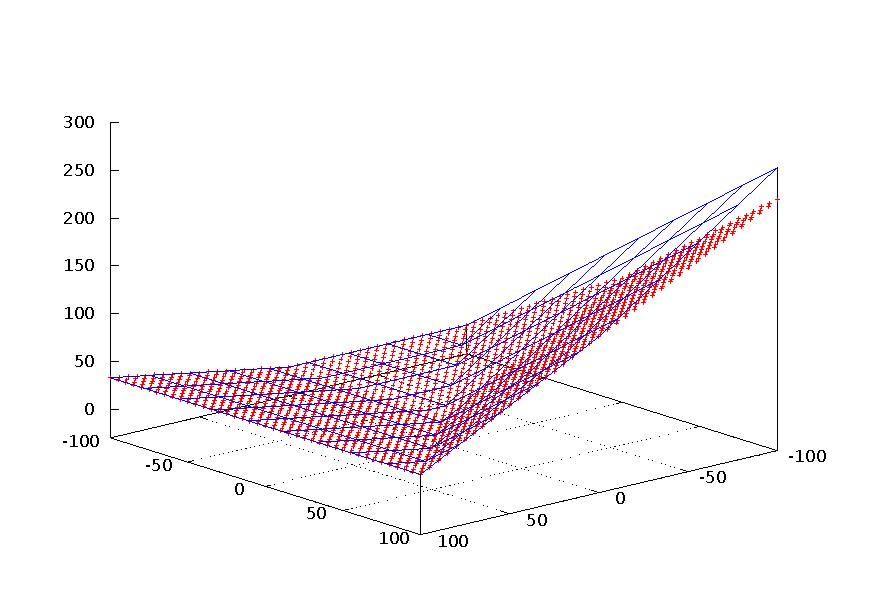
\includegraphics[width=\linewidth]{fig/bound3d}
\caption{The automatically derived bound $1.33|[x,y]| + 0.33 |[0,x]|$
  (blue lines) and the measured runtime cost (red crosses) for example
  \emph{t08a}. For $x\ge 0$ the derived bound is tight.}
\label{fig:3d}
\end{figure}

\section{Related Work}

Most closely related to this article is our previous work on
end-to-end stack-bound verification of Clight
programs~\cite{veristack14}.  In that work, we have implemented and
verified a quantitative logic to reason about stack-space usage.  In
this article, we present a more general quantitative Hoare logic that
is parametric in the resource of interest.  The main innovation over
our previous work~\cite{veristack14} is the novel automatic amortized
analysis for Clight programs that competes logical derivations for
non-trivial bounds for programs with loops and recursion.

Our work has been inspired by type-based amortized resource analysis
for functional programs~\cite{Jost03,HoffmannH10,HoffmannAH12}.  There
are three major improvements over previous work in the current paper,
which presents the first automatic amortized resource analysis for C.
First, we solved the long-standing open problem of extending automatic
amortized resource analysis to compute bounds for programs that loop
on (possibly negative) integers.  Second, we extended the analysis
system to deal with non-linear control flow that is introduced by
\code{break} and \code{return} statements.  Third, for the first time,
we combined an automatic amortized analysis with a system for
interactively deriving bounds.

In the development of our quantitative Hoare logic we have drawn
inspiration from mechanically verified Hoare logics.
Nipkow's~\cite{Nipkow02} description of his implementations of Hoare
logics in Isabelle/HOL has been helpful to understand the interaction
of auxiliary variables with the consequence rule.  Appel's separation
logic for CompCert Clight~\cite{AppelLogic} has been a blueprint for
the general structure of the quantitative logic.  Since we do not deal
with memory safety, our logic is much simpler and it would be possible
to integrate it with Appel's logic.  The continuation passing style
that we use in the quantitative logic is not only used by
Appel~\cite{AppelLogic} but also in Hoare logics for low-level
code~\cite{NiS06,JensenBK13}.

There exist quantitative logics that are integrated into separation
logic~\cite{Atkey10,HoffmannMZ13} and they are closely related to our
quantitative logic.  However, the purpose of these logics is slightly
different since they focus on the verification of bounds that depend
on the shape of heap data structures and they are not implemented for
C.  Also closely related to our logic is a VDM-style logic for
reasoning about resource usage of an abstract fragment of JVM byte
code by Aspinall et al.~\cite{AspinallBHLM07}.  Their logic is not
Hoare-style, does not target C code, and has been mainly designed to
produce certificates for bounds derived for high-level functional
programs.

There exist many tools that can automatically derive loops and
recursion bounds for imperative programs such as
SPEED~\cite{GulwaniMC09,GulwaniZ10}, KoAT~\cite{BrockschmidtEFFG14},
PUBS~\cite{AlbertAGPZ12}, Rank~\cite{AliasDFG10},
ABC~\cite{BlancHHK10} and LOOPUS~\cite{Zuleger11,SinnZV14}.  These
tools are based on abstract interpretation--based invariant generation
and/or term rewriting techniques, and they derive impressive results
on realistic software.  The importance of amortization to derive tight
bounds is well known in the resource analysis
community~\cite{AlonsoG12,Moser14,SinnZV14}.  Currently, the only
other available tools that can be directly applied to C code are Rank
and LOOPUS.  Our analysis framework does not aim to set a new standard
for automatic bound analysis.  Our contribution is rather a principled
approach that produces certificates that are proved sound with respect
to a formal cost semantics.  Moreover, we have a system that enables
both automatic and interactive bound derivation, a formal soundness
proof in Coq, and a method that can handle resources that can be
released (e.g., memory).  However, as we have shown
in~\pref{sec:exper}, our automatic amortized analysis matches that the
state of the art in automatic bound analysis for linear bounds and
sometimes even derives better constant factors than the other tools.
Since Rank and Loopus do not handle recursion, our automatic amortized
analysis is also the only available tool that can derive bounds for
recursive C programs.

There are techniques~\cite{Braberman08} that can compute the memory
requirements of object oriented programs with region based garbage
collection.  These systems infer invariants and use external tools
that count the number of integer points in the corresponding polytopes
to obtain bonds.  The described technique can handle loops but not
recursive or composed functions.

We are only aware of two verified quantitative analysis systems.
Albert et al.~\cite{AlbertBGHR12} rely on the KeY tool to
automatically verify previously inferred loop invariants, size
relations, and ranking functions for Java Card programs.  However,
they do not have a formal cost semantics and do not prove the bounds
correct with respect to a cost model.  Blazy et al.~\cite{Blazy13}
have verified a loop bound analysis for CompCert's RTL intermediate
language.  However, there is no way to interactively derive bounds or
to deal with resources like memory usage.  Also Blazy et al.'s
automatic bound analysis does not compute symbolic bounds.


\section{Conclusion}

We have introduced an novel quantitative analysis system for CompCert
Clight programs.  To the best of our knowledge, this article presents
the first resource analysis framework for C that makes it possible to
combine non-trivial automatically derived bounds with interactively
derived bounds in a proof system that produces verifiable certificates
for the bounds.  The main technical innovations are a quantitative
Hoare logic for reasoning about user-defined resource cost and an
automatic amortized analysis that derives bounds for programs whose
resource consumption depends on (possibly negative) integers and
non-sequential control flow as introduced by \code{break} and
\code{return} statements.

We will continue to improve our framework with the goal of reasoning
about resource usage of system software such as the hypervisor kernel
CertiKOS~\cite{GuVFSC11}, which we are currently developing and
verifying.  For on thing, we will improve the automation to derive
\emph{polynomial bounds} and to handle non-linear size changes, as
already developed for functional programs~\cite{HoffmannS13}.  For
another thing, we will build on previous work~\cite{HoffmannMZ13}
the generalize the quantitative Hoare logic to handle \emph{concurrent
  programs} with locks and lock-free data structures.

% \acks

% This research is based on work supported in part by NSF grants 1319671
% and 1065451, and DARPA grants FA8750-10-2-0254 and FA8750-12-2-0293.
% Any opinions, findings, and conclusions contained in this document are
% those of the authors and do not reflect the views of these agencies.

\clearpage
\appendix

\section{Catalog of Automatically Analyzed Programs}
\label{app:cat}

In this appendix we provide a non-exhaustive catalog of classes of
programs that can be automatically analyzed by our system.  For
simplicity, we use a cost metric that counts cost $1$ for assignments
and cost $0$ for all other operations.  Sometimes we also use the
\emph{ticks metric} if we want to discuss features like returning
resources.  Of course, the examples can also be analyzed with any other
cost metric.

We assume that free variables in the code snippets are the inputs to
the program. Some of the examples contain constants on which the
computed bound depends.  These constants are randomly chosen to
present an example but the analysis works for other constants as well.
Note however that it is sometimes crucial that constants are positive
(or negative) and that the same constant at different places.


\begin{figure*}[t!]
\setlength{\progwidth}{.24\linewidth}
  \centering

  \begin{minipage}[b]{\progwidth}
    \begin{center}
   \begin{lstlisting}
  while (z-y>0) {
    y = y+1;
  }
  while (y>9) {
    y=y-10;
  }
   \end{lstlisting}

$1.1|[y,z]| + 0.1|[0,y]|$
\\[.7\baselineskip] 
      {\bf t08}
    \end{center}
  \end{minipage}
%
%
%
  \begin{minipage}[b]{\progwidth}
    \begin{center}
   \begin{lstlisting}
  while (x-y>0) {
    if (*)
      y=y+1;
    else
      x=x-1;
  }
   \end{lstlisting}

$|[y,x]|$
\\[.7\baselineskip]
      {\bf t10}
    \end{center}
  \end{minipage}
%
%
%
  \begin{minipage}[b]{\progwidth}
    \begin{center}
   \begin{lstlisting}
  while (x>0) {
    x=x-1;
    if (*) 
      y=y+1;
    else {
      while (y>0)
        y=y-1;
    }
  }
   \end{lstlisting}

$3|[0,x]| + |[0,y]|$
\\[.7\baselineskip]
      {\bf t13}
    \end{center}
  \end{minipage}
%
%
%
  \begin{minipage}[b]{\progwidth}
    \begin{center}
   \begin{lstlisting}
while (n<0) {
  n=n+1;
  y=y+1000;
  while (y>=100 && *){
    y=y-100;
  }
}
   \end{lstlisting}

$12|[n,0]| + 0.01|[0,y]|$
\\[.7\baselineskip]
      {\bf t27}
    \end{center}
  \end{minipage}
   \caption{Amortization and Compositionality (a)}
  \label{fig:cat1a}
\end{figure*}


\begin{figure*}[t!]
 \setlength{\progwidth}{.24\linewidth}
  \centering

  \begin{minipage}[b]{\progwidth}
    \begin{center}
   \begin{lstlisting}
  while (x>0) {
    x=x-1;
    y=y+2;
  }
  while (y>0) {
    y=y-1;
  }
  while (y>0) {
    y=y+1;
  }
   \end{lstlisting}

$4|[0,x]| + |[0,y]|$
\\[.7\baselineskip]
      {\bf t07}
    \end{center}
  \end{minipage}%
%
%
%
  \begin{minipage}[b]{\progwidth}
    \begin{center}
   \begin{lstlisting}
  while (x>y) {
    x=x-1;
    x=x+1000;
    y=y+1000;
  }
  while (y>0) {
    y=y-1;
  }
  while (x<0) {
    x=x+1;
  }
   \end{lstlisting}

$1004|[y,x]|+|[x,0]|+|[0,y]|$
\\[.7\baselineskip]
      {\bf t28}
    \end{center}
  \end{minipage}%
%
%
  \begin{minipage}[b]{\progwidth}
    \begin{center}
   \begin{lstlisting}
  assert (y>=0);
  while (x-y>0) {
    x=x-1;
    x=x-y;
    z=y;
    while (z>0) {
      z=z-1;
    }
  }
   \end{lstlisting}

$3|[0,x]|$
\\[.7\baselineskip]
      {\bf t15}
    \end{center}
  \end{minipage}
%
%
  \begin{minipage}[b]{\progwidth}
    \begin{center}
   \begin{lstlisting}
  assert (y>=0);
  while (x-y>0) {
    x=x-1;
    x=x-y;
    z=y;
    z=z+y;
    z=z+100;
    while (z>0) {
      z=z-1;
    }
  }
   \end{lstlisting}

$1+2|[0,x]|+103|[y,x]|$
\\[.7\baselineskip]
      {\bf t16}
    \end{center}
  \end{minipage}


   \caption{Amortization and Compositionality (b)}
  \label{fig:cat1b}
\end{figure*}


\begin{figure*}[t!]
 \setlength{\progwidth}{.24\linewidth}
  \centering

  \begin{minipage}[b]{\progwidth}
    \begin{center}
   \begin{lstlisting}
  while (i>100) {
    i--;
  }
  i=i+k+50;
  while (i>=0) {
    i--;
  }
   \end{lstlisting}

$52 + |[-1,i]| + |[0,k]|$
\\[.7\baselineskip]
      {\bf t19}
    \end{center}
  \end{minipage}%
%
%
%
  \begin{minipage}[b]{\progwidth}
    \begin{center}
   \begin{lstlisting}
  while (x<y) {
    x=x+1;
  }
  while (y<x) {
    y=y+1;
  }
   \end{lstlisting}

$|[x,y]|+|[y,x]|$
\\[.7\baselineskip]
      {\bf t20}
    \end{center}
  \end{minipage}%
%
%
  \begin{minipage}[b]{\progwidth}
    \begin{center}
   \begin{lstlisting}
  while (x>0) {
    x=x-1;
    t=x;
    x=y;
    y=t;
  }
   \end{lstlisting}

$4|[0,x]|+4|[0,y]|$
\\[.7\baselineskip]
      {\bf t30}
    \end{center}
  \end{minipage}
%
%
  \begin{minipage}[b]{\progwidth}
    \begin{center}
   \begin{lstlisting}
  flag=1;
  while (flag>0) {
    if (n>0 && *) {
      n=n-1;
      flag=1;
    } else
      flag=0;
  }
   \end{lstlisting}

$2 + 2|[0, n]|$
\\[.7\baselineskip]
      {\bf t47}
    \end{center}
  \end{minipage}

   \caption{Amortization and Compositionality (c)}
  \label{fig:cat1c}
\end{figure*}

\paragraph{Amortization and Compositionality}

Figures~\ref{fig:cat1a}, \ref{fig:cat1b}, and~\ref{fig:cat1c} show
code snippets that need amortization are compositionality to obtain a
whole program bound.

Example \emph{t07} demonstrates two different features of the
analysis.  For one thing it shows that we can precisely track size
changes inside loops.  In the first loop, we increment $y$ by $2$ in
each of the $|[0,x]|$ iterations.  An in the second loop, we decrement
$y$.  For another thing it shows that we automatically recognize dead
code if we find conflicting assertions on a branching path: After the
second loop we know $y \leq 0$ and as a result can assign arbitrary
potential inside the third loop where we know that $y>0$.  As a
result, we obtain a tight bound.

Example \emph{t08} shows the ability of the analysis to handle
negative and non-negative numbers.  Note that there are no
restrictions on the signs of $z$ and $y$.  We also see again that we
accurately track the size change of $y$ in the first loop.
Furthermore, \emph{t08} shows that we do not handle the constants $1$
or $0$ in any special way.  In all examples you could replace $0$ and
$1$ with other constants like we did in the second loop and still
derive a tight bound.  The only information, that the analyzer needs
is $y \geq c$ before assigning $y = y - c$.

In example \emph{t10} we also do not restrict the inputs $x$ and $y$.
They can be negative, positive, or zero.  The star {\tt *} in the
conditional, stands for an arbitrary assertion.  In each branch of the
conditional we can obtain the constant potential $1$ since the interval
size $|[y,x]|$ is decreasing.

Example \emph{t13} shows how amortization can be used to handle tricky
nested loops.  The outer loop is iterated $|[0,x]|$ times.  In the
conditional, we either (the branching condition is again arbitrary)
increment the variable $y$ or we execute an inner loop in which $y$ is
counted back to $0$.  The analysis computes a tight linear bound for
this program.  Again, the constants $0$ and $1$ in the inner loop can
as well be replace by something more interesting, say $9$ and $10$
like in example \emph{t08}.  Then we still obtain a tight linear
bound.

Example \emph{t27} is similar to example \emph{t13}.  Instead of
decrementing the variable $x$ in the outer loop we this time increment
the variable $n$ till $n = 0$.  In each of the $|[n,0]|$ iterations,
we increment the variable $y$ by $1000$.  We then execute an inner
loop that increments $y$ by $100$ until $y=0$.  The analysis can
derive that only the first execution of the inner loop depends on the
initial value of $y$.  We again derive a tight bound.

Example \emph{t28} is particularly interesting.  In the first loop we
decrement the size $|[y,x]|$.  However, we also shift the interval
$[y,x]$ to the interval $[y+1000,x+1000]$.  The analysis can derive
that this does not change the size of the interval and computes the
tight loop bound $3|[y,x]|$.  The additional two loops are in the
program to show that the size tracking in the first loop works
accurately.  The second loop is executed $|[0,y]| + 1000|[y,x]|$ times
in the worst case.  The third loop is executed $|[x,0]| + |[y,x]|$ in
the worst case (if $x$ and $y$ are negative).

Sometimes we need some assumptions on the inputs in order to derive a
bound.  Example \emph{t15} is such a case.  We assume here that the
input variable $y$ is non-negative and write \code{assert(y>=0)}.  The
semantic of \code{assert} is that it has no effect if the assertion is
true and that the program is terminated without further cost
otherwise.  If we enter the loop then we know that $x>0$ and we can
obtain constant potential from the assignment \code{x=x-1}.  After the
assignment we know that $x\geq y$ and $y\geq 0$.  As a consequence, we
can share the potential $3|[0,x]|$ before the assignment \code{x=x-y}
between $3|[0,x]|$ and $3|0,y|$ after the assignment.  In this way, we
derive a tight linear bound.

Example \emph{t16} is an extension of example \emph{t15}. We again
assume that $y$ is non-negative and use the same mechanism to iterate
the outer loop as in \emph{t15}.  In the inner loop, we also count the
variable $z$ down to zero and perform $|[0,z]|$ interations.  However,
instead of assigning \code{z=y}, we assign \code{z=2y+100}.  The analysis
computes the tight linear bound $1+2|[0,x]|+103|[y,x]|$.  The
assignment of potential to the size interval $|[y,x]|$ in instead of
$|[0,x]|$ is a random choice of the LP solver.  Other optimal
solutions of the linear program that the analyzer gernerates for
\emph{t15} would result in bounds such as $1+105|[0,x]|$ or
$1+6|[0,x]|+99|[y,x]|$.  In fact, the $105$ potential units can be
shared arbitrarily between the interval sizes $|[y,x]|$ and $|[0,x]|$
as long as more than $1$ unit is assigned to $|[0,x]|$.  Since we know
that, $y\geq 0$ the choice of the LP solver is optimal but this seems
to be a coincidence.

Example \emph{t19} demonstrates another nice property that demonstates
the compositionaliy of the analysis.  The program consists of two
loops that decrement a variable $i$.  In the first loop, $i$ is
decremented down to 100 and in the second loop $i$ is increment
further down to $-1$.  However, between the loops we assign
$i=i+k+50$.  So in total the program performs $52 + |[-1,i]| +
|[0,k]|$ increments.  Our analysis finds this tight bound because our
amortized analysis naturally takes into account the relation between
the two loops.  Other techniques might derive a more conservative
bound such as $52 + |[-1,i]| + |[0,k]| + |[100,i]|$.

Example \emph{t20} shows how we can handle programs in which bounds
contain absolute values like $|x-y|$.  The first loop body is only
executed if $x<y$ and the second loop body is only executed if $y<x$.
The analyzer finds a tight bound.

At first sight, example \emph{t30} appears to be a simple loop that
decrements the variable $x$ down to zero.  However, a closer look
reveals that the loop actually decrements both input variables $x$ and
$y$ down to zero before terminating.  In the loop body, first $x$ is
decremented by one.  Then the values of the variables $x$ and $y$ are
switched using the local variable $t$ as a buffer.  Our analysis
infers the tight bound $4|[0,x]|+4|[0,y]|$.

Example \emph{t47} demonstrates how we can use integers as Booleans to
amortize the cost of loops that depend on boolean flags.  The outer
loop is executed as long as the variable flag is ``true'', that is,
\code{flag>0}.  Inside the loop, there is a conditional that either
(if $n>0$) decrements $n$ and assigns \code{flag=1}, or (if $n\geq0$)
leaves n unchanged and assigns \code{flag=0}.  The analyzer computes
the tight bound $2 + 2|[0, n]|$.  The potential in the loop invariant
is $|[0,\mathit{flag}]| + 2|[0, n]|$.  In the \emph{then} branch of
the conditional, we use the potential $2|[0, n]|$ and the fact that
$n>0$.  In the \emph{else} branch, we use the potential
$|[0,\mathit{flag}]|$ and the fact that $\mathit{flag}=1$.




\begin{figure*}[t!]
 \setlength{\progwidth}{.24\linewidth}
  \centering
  \begin{minipage}[b]{\progwidth}
    \begin{center}
   \begin{lstlisting}
  while (n>x) {
    if (m>y) 
      y = y+1;
    else
      x = x+1;
  }
   \end{lstlisting}

$|[x, n]| + |[y, m]|$
\\[.7\baselineskip]
      {\bf fig2\_1}
    \end{center}
  \end{minipage}
%
%
  \begin{minipage}[b]{\progwidth}
    \begin{center}
   \begin{lstlisting}
  while (x<n) {
    if (z>x)
      x=x+1;
    else
      z=z+1;
  }
   \end{lstlisting}

$|[x, n]| + |[z, n]|$
\\[.7\baselineskip]
      {\bf fig2\_2}
    \end{center}
  \end{minipage}
%
%
  \begin{minipage}[b]{\progwidth}
    \begin{center}
   \begin{lstlisting}
  while (x<n) {
    while (y<m) {
      if (*) break;
      y=y+1;
    }
    x=x+1;
  }
   \end{lstlisting}

$|[x, n]| + |[y, m]|$
\\[.7\baselineskip]
      {\bf nested\_multiple}
    \end{center}
  \end{minipage}
%
%
  \begin{minipage}[b]{\progwidth}
    \begin{center}
   \begin{lstlisting}
  x=0;
  while (x<n) {
    x=x+1;
    while (x<n) {
      if (*) break;
      x=x+1;
    }
  }
   \end{lstlisting}

$1 + |[0, n]|$
\\[.7\baselineskip]
      {\bf nested\_single}
    \end{center}
  \end{minipage}

   \caption{Examples from Gulwani et al's SPEED~\cite{GulwaniMC09}} (a)
  \label{fig:cat2a}
\end{figure*}

\begin{figure*}[t!]
 \setlength{\progwidth}{.24\linewidth}
  \centering
  \begin{minipage}[b]{\progwidth}
    \begin{center}
   \begin{lstlisting}
  x=0;
  while (x<n) {
    if (*) break;
    x=x+1;
  }
  while (x<n)
    x=x+1;
   \end{lstlisting}

$1 + |[0,n]|$
\\[.7\baselineskip]
      {\bf sequential\_single}
    \end{center}
  \end{minipage}
%
%
  \begin{minipage}[b]{\progwidth}
    \begin{center}
   \begin{lstlisting}
  x=0; y=0;
  while (x<n) {
    if (y<m)
      y=y+1;
    else
      x=x+1;
  }
   \end{lstlisting}
$2 + |[0, m]| + |[0, n]|$
\\[.7\baselineskip]
      {\bf simple\_multiple}
    \end{center}
  \end{minipage}
%
%
  \begin{minipage}[b]{\progwidth}
    \begin{center}
   \begin{lstlisting}
  x=0;
  while (x<n) {
    if (*)
      x=x+1;
    else 
      x=x+1;
  }
   \end{lstlisting}

$1 + |[0,n]|$
\\[.7\baselineskip]
      {\bf simple\_single}
    \end{center}
  \end{minipage}
%
%
  \begin{minipage}[b]{\progwidth}
    \begin{center}
   \begin{lstlisting}
  x=0; y=0;
  while (*) {
    if (x<N) {
      x=x+1; y=y+1;
    } else if (y<M ) {
      x=x+1; y=y+1;
    } else
      break;
  }
   \end{lstlisting}

$2 + 2 |[0, M]| + 2 |[0, N]|$
\\[.7\baselineskip]
      {\bf simple\_single\_2}
    \end{center}
  \end{minipage}

   \caption{Examples from Gulwani et al's SPEED~\cite{GulwaniMC09} (b)}
  \label{fig:cat2b}
\end{figure*}





\begin{figure*}[t!]
 \setlength{\progwidth}{.24\linewidth}
  \centering
%
%
  \begin{minipage}[b]{\progwidth}
    \begin{center}
   \begin{lstlisting}
  assert n>0;
  assert m>0;
  va = n; vb = 0;
  while (va>0 && *) {
    if (vb<m) { 
      vb=vb+1; 
      va=va-1;
    } else {
      vb=vb-1;
      vb=0;
    }
  }
   \end{lstlisting}
$2 + 4|[0, n]|$
\\[.7\baselineskip]
      {\bf fig4\_2}
    \end{center}
  \end{minipage}
%
%
%
%
  \begin{minipage}[b]{\progwidth}
    \begin{center}
   \begin{lstlisting}
  assert (0<m);
  i = n;
  while (i>0 && *) {
    if (i<m)
      i=i-1;
    else
      i=i-m;
  }
   \end{lstlisting}
$|[0, n]|$
\\[.7\baselineskip]
      {\bf fig4\_4}
    \end{center}
  \end{minipage}
%
%
  \begin{minipage}[b]{\progwidth}
    \begin{center}
   \begin{lstlisting}
  assert (0 < m < n);
  i=m;
  while (0<i<n) {
    if (dir==fwd) i++;
    else i--;
  }
   \end{lstlisting}
$---$
\\[.7\baselineskip]
      {\bf fig4\_5}
    \end{center}
  \end{minipage}

   \caption{Examples from [GulwaniPLDI09]}
  \label{fig:cat2c}
\end{figure*}


\begin{figure*}[t!]
 \setlength{\progwidth}{.24\linewidth}
  \centering
%
%
  \begin{minipage}[b]{\progwidth}
    \begin{center}
   \begin{lstlisting}
  i=0;
  while (i<n) {
    j=i+1;
    while (j<n) {
      if (*) {
        _tick(1);
        j=j-1; n=n-1;
      }
      j=j+1;
    }
    i=i+1;
  }
   \end{lstlisting}
$|[0, n]| \text{ ticks}$
\\[.7\baselineskip]
      {\bf ex1}
    \end{center}
  \end{minipage}
%
%
  \begin{minipage}[b]{\progwidth}
    \begin{center}
   \begin{lstlisting}
  while (n>0 && m>0) {
    n--; m--;
    while (nondet()) {
      n--; m++;
    }
  }
   \end{lstlisting}
$---$
\\[.7\baselineskip]
      {\bf ex2}
    \end{center}
  \end{minipage}
%
%
  \begin{minipage}[b]{\progwidth}
    \begin{center}
   \begin{lstlisting}
  while (n>0) {
    t = x;
    n=n-1;
    while (n>0) {
      if (*) break;
      n=n-1;
    }
  }
   \end{lstlisting}
$2 |[0, n]|$
\\[.7\baselineskip]
      {\bf ex3}
    \end{center}
  \end{minipage}
%
%
  \begin{minipage}[b]{\progwidth}
    \begin{center}
   \begin{lstlisting}
  flag=1;
  while (flag>0) {
    flag=0;
    while (n>0 && *) {
      n=n-1;       
      flag=1;
    }
  }
   \end{lstlisting}
$2 + 3|[0, n]|$
\\[.7\baselineskip]
      {\bf ex4}
    \end{center}
  \end{minipage}


   \caption{Examples from [GulwaniPLDI10]}
  \label{fig:cat3a}
\end{figure*}


\paragraph{From  the Literature}

Our analyzer can derive almost all linear bounds for programs that
have been described as challenges in the literature on bound
generation.  We found only three programs with a linear bound for
which our analyzer could not find a tight bound.  The first one
(\emph{fig4\_5}) from [GulwaniPLDI09] requires \emph{path-sensitive
  reasoning} to derive a bound.  The other two, \emph{ex2} and
\emph{ex5} (see [GulwaniPLDI10]), from [GulwaniPLDI10] were described
to have a linear bound but seem to be non-terminating.

Examples \emph{fig2\_1} and \emph{fig2\_2} are taken from Gulwani et
al~\cite{GulwaniMC09}.  They are both handled by the SPEED tool but
require inference of a \emph{disjunctive invariant}.  In the abstract
interpretation community, these invariants are known to be notoriously
difficult to handle.
%
In example \emph{fig2\_1} we have one loop that first increments
variable $y$ up to $m$ and then increments variable $x$ up to $n$.  We
derive the tight bound $|[x, n]| + |[y, m]|$.
%
Example \emph{fig2\_2} is more tricky and trying to understand how it
works may be challenging.  However, with the amortized analysis in
mind, using the potential transfer reasoning, it is almost trivial to
prove a bound.  While the SPEED tool has to find a fairly
involved invariant for the loop, our tool is simply reasoning locally
and works without any clever tricks. We obtain the tight bound $|[x,
n]| + |[z, n]|$.

Example \emph{nested\_multiple} is similar to example \emph{fig2\_1}.
Instead of incrementing variable $y$ in the outer loop, $y$ is here
potentially incremented multiple times in each iteration of the outer
loop.  The idea of example \emph{nested\_single} is similar.  However,
instead of incrementing variable $y$ in the inner loop, we increment
$x$, the counter variable of the outer loop. Our analyzer derives a
tight bound for both programs.  Note that a star \emph{*} in a
branching condition denotes an arbitrary boolean condition that might
of course change while iterating (non-deterministic choice).

Example \emph{sequential\_single} is like example
\emph{nested\_single}.  The only difference is that the inner loop of
\emph{nested\_single} is now evaluated after the outer loop.  Example
\emph{simple\_multiple} is a variant of example \emph{fig2\_1} and
\emph{simple\_single} is a simple variant of \emph{nested\_single}.
We derive tight bounds for all aforementioned programs.

Example \emph{simple\_single\_2} uses conditionals and a \code{break}
statement to control loop iterations.  If $x<N$ then variables $x$ and
$y$ are incremented.  Otherwise, if $y<M$ then the same increment is
executed.  If $y\geq M$ and $x\geq N$ then the loop is terminated with
a break.  Our tool computes the bound $2 + 2 |[0, M]| + 2 |[0, N]|$.
This bound is tight in the sense that there are inputs (such as $M =
-100$ and $N = 100$) for which the bound precisely describes the
execution cost.  However, SPEED can compute the more precise bound
$\max(N,M)$.  We currently cannot express this bound in our system.

Example \emph{fig4\_2} from [GulwaniPLDI09] is quite involved.
Amortized reasoning helps to understand how we derive the bound $4 +
4|[0, n]|$.  We start with potential $6 + 4|[0, n]|$ and use the
constant potential to pay for the two first assignments.  We use the
remaining potential $4 + 4|[0, n]|$ and the fact that $vb=0$ to
establish the potential $4 + 4|[0, n]| + 2|[0,vb]|$ that serves as a
loop invariant.  In the \emph{if branch} of the conditional, we use
the constant potential $4$ of the invariant to pay for the two
assignments ($2$ units) and the potential of $|[0,vb]|$ ($2$ units).
Since we also know that $|[0, n]|>0$ we obtain constant potential $4$
and establish the loop invariant again.  In the \emph{else} branch, we
use the potential $2|[0,vb]|$ and the fact $vb>0$ to obtain $2$
potential units to pay for the assignment.  Since we have $4$ constant
potential units left after the loop, we can subtract them from the
initial potential $6 + 4|[0, n]|$.

In example \emph{fig4\_4} it is essential that $m$ is positive.
That ensures that we can obtain constant potential for the interval
size $|[0,i]|$ in the \emph{else} branch of the conditional since
$|[0,i]|$ decreases.  Example \emph{fig4\_5} is one of the three
examples that we can not handle automatically.  The execution is
bounded because the boolean value of the test \code{dir==fwd} does not
change during the iteration of the loop.  As a result, the variable
$i$ is either counted down to $0$ or up to $n$.  Our tool cannot
handle example \emph{fig4\_5} because we don't do path sensitive
reasoning.  Note however that it would be more efficient to move the
test \code{dir==fwd} outside of the loop (this would be also done by
an optimizing compiler).  The resulting program could be analyzer by our
tool.

Example \emph{ex1} from [GulwaniPLDI10] specifically focusses on the
code in the \emph{if} statement.  So we use the \emph{tick metric} and
insert \code{_tick(1)} inside the if statement to derive a bound on
the number of times the code in the if statement is executed.  Note
that we cannot derive a bound for the whole program since the outer
loop is executed a quadratic number of times.  Nevertheless it is
straightforward to derive a bound on the number of ticks using the
amortized approach: In the if statement we know that $n>0$ and assign
\code{n=n-1}.  So we can use the potential of the interval size $|[0,n]|$
to pay for the tick.

We cannot analyze example \emph{ex2} for which previous work reported
a linear bound [GulwaniPLDI10].  The reason is that this example is
not terminating since the inner loop is not bounded.  The same is true
for example \emph{ex5} from the same paper, which is not listed here.
Finally, example \emph{ex2} is similar to example
\emph{nested\_single}, and \emph{ex3} is a variant of example
\emph{t47}.

\begin{figure*}[t!]
 \setlength{\progwidth}{.28\linewidth}
  \centering
%
%
  \begin{minipage}[b]{\progwidth}
    \begin{center}
   \begin{lstlisting}
void count_down (int x) {
  int a = x;
  if (a>0) {
    a = a-1;
    count_down(a);
  }
}
int copy (int x, int y) {
  if (x>0) {
    x = x-1;
    y = y+1;
    y=copy(x,y);
  };
  return y;
}
void _main (int x,int y) {
  y = copy (x,y);
  count_down(y);
}
   \end{lstlisting}

$1 + 4|[0, x]| + 2|[0, y]|$
\\[.7\baselineskip]
      {\bf t37}
    \end{center}
  \end{minipage}
%
%
  \begin{minipage}[b]{\progwidth}
    \begin{center}
   \begin{lstlisting}
void count_down (int x,int y)
{ int a = x;
  if (a>y) {
    a = a-1;
    count_up(a,y);
  }
}

void count_up (int x, int y)
{ int a = y;
  if (a+1<x) {
    a = a+2;
    count_down(x,a);
  }
}

void _main (int y, int z) {
  count_down(y,z);
}
   \end{lstlisting}

$1.67 + 1.33 |[z,y]|$
\\[.7\baselineskip]
      {\bf t39}
    \end{center}
  \end{minipage}
%
%
  \begin{minipage}[b]{\progwidth}
    \begin{center}
   \begin{lstlisting}
void produce () {
  while (x>0) {
    _tick(-1); x=x-1; y=y+1;
  }
}
void consume () {
  while (y>0) {
    y=y-1; x=x+1; _tick(1);
  }
}
void _main (int y, int z) {
  consume(); produce(); consume();
}
   \end{lstlisting}

$|[0, y]|$ ticks
\\[.7\baselineskip]
      {\bf t46}
    \end{center}
  \end{minipage}

   \caption{Programs with (recursive) functions}
  \label{fig:cat3}
\end{figure*}


\paragraph{Recursive Functions}

Our approach can naturally deal with mutually-recursive functions.
The recursion patterns can be exactly the same that are used in
iterations of loops.  In the following, we present three simple
examples that illustrate the analysis of functions.

Example \emph{t37} illustrates that the analyzer is able to perform
inter-procedural size tracking.  The function \code{copy} adds the
argument $x$ to the argument $y$ if $x$ is positive.  However, this
addition is done in steps of $1$ in each recursive call.  The function
\code{count\_down} recursively decrements its argument down to $0$.
The derived bound $1 + 4|[0, x]| + 2|[0, y]|$ is for the function
\code{\_main} in which we first add $x$ to $y$ using the function
\code{copy} and then count down the variable $y$ using the function
\code{count\_down}.  The derived bound is tight.

Example \emph{t39} uses mutual recursion.  The function
\code{count\_down} is similar to the function with the same name in
example \emph{t37}.  However, we do not count down to $0$ but to a
variable $y$ that is passed as an argument and we call the function
\code{count\_up} afterwards.  The function \code{count\_up} is dual to
\code{count\_down}.  Here, we count up $y$ by $2$ and recursively call
\code{count\_down}.  For the function $\_main$, which calls
\code{count\_down(y,z)}, the analyzer computes the tight bound $1.67 +
1.33 |[z,y]|$.

Example \emph{t46} shows a program that uses and returns resources.
Again, we use the \emph{tick metric} and the function \code{\_tick} to
describe the resource usage.  The function \code{produce} produces
$|[0,x]|$ resources, that is, in each of the $|[0,x]|$ iterations, it
receives one resource unit.  Similarly, the function \code{consume}
consumes $|[0,y]|$ resources.  The analyzer computes the tight bound
$|[0,y]|$ for the function \code{\_main}.  This is only possible since
amortized analysis naturally tracks the size changes to the variables
$x$ and $y$, and the interaction between \code{consume} and
\code{produce}.


\begin{figure*}[t!]
 \setlength{\progwidth}{.32\linewidth}
  \centering
%
%
  \begin{minipage}[b]{\progwidth}
    \begin{center}
   \begin{lstlisting}
int srch(
  int t[], int n,  /* haystack */
  int p[], int m,  /* needle */
  int b[]
) {
  int i=0, j=0, k=-1;

  while (i < n) {
    while (j >= 0 && t[i]!=p[j]) {
      k = b[j];
      assert(k > 0);
      assert(k <= j + 1);
      j -= k;
    }
    i++, j++;
    if (j == m)
      break;
  }
  return i;
}
   \end{lstlisting}

$1 + 2|\inter 0 n|$
\\[.7\baselineskip]
      {\bf Knuth-Morris-Pratt}
    \end{center}
  \end{minipage}
%
%
  \begin{minipage}[b]{\progwidth}
    \begin{center}
   \begin{lstlisting}
int gcd(int x, int y) {
  if (x <= 0) return y;
  if (y <= 0) return x;

  for (;;) {
    if (x>y) x -= y;
    else if (y>x) y -= x;
    else return x;
  }
}
   \end{lstlisting}

$|\inter 0 x| + |\inter 0 y|$
\\[.7\baselineskip]
      {\bf Greatest Common Divisor}
    \end{center}
  \end{minipage}
%
%
  \begin{minipage}[b]{\progwidth}
    \begin{center}
   \begin{lstlisting}
void qsort(int a[], int lo, int hi) {
  int m1, m2, n;

  if (hi - lo < 1) return;

  n = nondet(); /* partition the array */
  assert( n > 0 );
  assert( lo + n <= hi );

  m1 = n + lo;
  m2 = m1 - 1;

  qsort(a, m1, hi);
  qsort(a, lo, m2);
}

void main(int a[], int len) {
  qsort(a, 0, len);
}
   \end{lstlisting}

$1 + 2 |\inter 0 {\code{len}}|$
\\[.7\baselineskip]
      {\bf Quick Sort}
    \end{center}
  \end{minipage}

   \caption{Well-Known Algorithms}
  \label{fig:cat3}
\end{figure*}

\paragraph{Well-Known Algorithms}



\begin{figure*}
\small

\newcommand{\dir}[2]{\texttt{#1} \\ \texttt{#2}}
\newcommand{\file}[2][c]{%
  \begin{tabular}[#1]{@{}r@{}}#2\end{tabular}}
\renewcommand{\max}[0]{{\rm mx}}
\renewcommand{\min}[0]{{\rm mn}}

\newcolumntype{C}[1]{>{\centering\let\newline\\\arraybackslash\hspace{0pt}}m{#1}}

\centering
\begin{tabular}{r|C{1.1cm}c|C{1.8cm}c|C{1.9cm}c|C{1.8cm}|C{2.65cm}}

 
File &
\multicolumn{2}{|c|}{KoAT} &
\multicolumn{2}{|c|}{Rank} &
\multicolumn{2}{|c|}{Loopus} &
Speed &
Amortized Automation
\\
\hline

%--------------------------------------------
\hline \texttt{gcd.c} &

? &
&

% $((((1+1)+1)+((-5+(2{\cdot}y))+(2{\cdot}x)))+(-3+(2{\cdot}y)))+1$ &
$(((2{+}1)\dots$ &
$O(n)$ &

--- &
&

? &

$|\inter 0 x| {+} |\inter 0 y|$
\\

%--------------------------------------------
\hline \texttt{kmp.c} &

? &
&

% $((((1+1)+(n+(-1{\cdot}i)))+((n+(n{\cdot}j))+((-1+(-1{\cdot}j)){\cdot}i)))+((n+(n{\cdot}j))+((-1+(-1{\cdot}j)){\cdot}i)))+1$ &
$(((2{+}(n{+} \dots$ &
$O(n^2)$ &

% $\max(n, 0) + \max(0, (1 + \max(n, 0))) + \max(0, (1 + \max(n, 0)))$ &
$\max(n, 0) \dots$ &
$O(n)$ &

? &

$1 {+} 2 |\inter 0 n|$
\\

%--------------------------------------------
\hline \texttt{qsort.c} &

? &
&

--- &
&

--- &
&

? &

$1 {+} 2 |\inter 0 {\code{len}}|$
\\

%--------------------------------------------
% \hline \file{\dir{speed\_pldi09}{fig1.c}} &
% 
% ? &
% &
% 
% --- &
% &
% 
% $2 \max(n, 0)$ &
% $O(n)$ &
% 
% God damn it &
% 
% $1 + 2 |\inter 0 n|$
% \\

%--------------------------------------------
\hline \file{\dir{speed\_pldi09}{fig4\_2.c}} &

--- &
&

% $((((1+1)+n)+(n+(-1{\cdot}m)))+1)+1$ &
$(((2{+}n)\dots$ &
$O(n)$ &

--- &
&

$\frac n m + n$ &

$1 {+} 2 |\inter 0 n|$
\\

%--------------------------------------------
\hline \file{\dir{speed\_pldi09}{fig4\_4.c}} &

--- &
&

% $((((1+1)+(-1+m))+((1+n)+(-1{\cdot}m)))+1)+1$ &
$(((2{+}(-1\dots$ &
$O(n)$ &

--- &
&

$\frac n m + n$ &

$|\inter 0 n|$
\\

%--------------------------------------------
\hline \file{\dir{speed\_pldi09}{fig4\_5.c}} &

$28d + 7g + 27$ &
$O(n)$ &

% $((((1+1)+(-1+n))+m)+1)+1$ &
$(((2{+}(-1\dots$ &
$O(n)$ &

--- &
&

$\max(n, n-m)$ &

---
\\

%--------------------------------------------
\hline \file{\dir{speed\_pldi10}{ex1.c}} &

--- &
&

--- &
&

--- &
&

$n$ &

$|\inter 0 n|$
\\

%--------------------------------------------
\hline \file{\dir{speed\_pldi10}{ex3.c}} &

--- &
&

% $((((1+1)+(-1+n))+(-1+n))+1)+1$ &
$(((2{+}(-1\dots$ &
$O(n)$ &

$2{\cdot}\max(n, 0)$ &
$O(n)$ &

$n$ &

$|\inter 0 n|$
\\

%--------------------------------------------
\hline \file{\dir{speed\_pldi10}{ex4.c}} &

$110 a + 33$ &
$O(n)$ &

--- &
&

--- &
&

$n + 1$ &

$1 {+} 2 |\inter 0 n|$
\\

%--------------------------------------------
\hline \file{\dir{speed\_popl10}{fig2\_1.c}} &

$9a + 9b + \dots$ &
$O(n)$ &

% $(((1+1)+((-1{\cdot}y)+m))+((-1{\cdot}x)+n))+1$ &
$((2{+}((-y\dots$ &
$O(n)$ &

$\max(0, n {-} x) + \max(0, m {-} y)$ &
$O(n)$ &

$\max(0, n{-}x) + \max(0, m{-}y)$ &

$|\inter x n| {+} |\inter y m|$
\\

%--------------------------------------------
\hline \file{\dir{speed\_popl10}{fig2\_2.c}} &

$6a + 9b + 3c + 5$ &
$O(n)$ &

% $(((1+1)+((-1{\cdot}x)+n))+(((-1+(-1{\cdot}z))+(-1{\cdot}x))+(2{\cdot}n)))+1$ &
$((2{-}x\dots$ &
$O(n)$ &

% $\max(0, (\max(0, (x {+} 1 {+} -z)) + \max(0, (n - x)))) + \max(0, (n - x))$ &
$\max(0, (x + 1 {-}z)\dots$ &
$O(n)$ &

$\max(0, n{-}x) + \max(0, n{-}z)$ &

$|\inter x n| {+} |\inter z n|$
\\

%--------------------------------------------
\hline \file{\dir{speed\_popl10}{nstd\_multiple.c}} &

--- &
&

% $(((1+1)+((-1{\cdot}x)+n))+(((y{\cdot}x)+((-1{\cdot}y){\cdot}n))+(((-1{\cdot}x)+n){\cdot}m)))+1$ &
$((2{-}x{+}n\dots$ &
$O(n^2)$ &

$\max(0, m {-} y) + \max(0, n {-} x)$ &
$O(n)$ &

$\max(0, m{-}y) + \max(0, n{-}x)$ &

$|\inter x n| {+} |\inter y m|$
\\

%--------------------------------------------
\hline \file{\dir{speed\_popl10}{nstd\_single.c}} &

$48 b + 16$ &
$O(n)$ &

% $((((1+1)+((-1+(-1{\cdot}x))+n))+((-1+(-1{\cdot}x))+n))+1)+1$ &
$(((1{-}x{+}n\dots$ &
$O(n)$ &

$\max(0, \! n {-} 1)\dots$ &
$O(n)$ &

$n$ &

$|\inter 0 n|$
\\

%--------------------------------------------
\hline \file{\dir{speed\_popl10}{sqntl\_single.c}} &

$21 b + 6$ &
$O(n)$ &

% $(((1+1)+((-1{\cdot}x)+n))+((-1{\cdot}x)+n))+1$ &
$((2{}-x{+}n\dots$ &
$O(n)$ &

$2{\cdot}\max(n, 0)$ &
$O(n)$ &

$n$ &

$|\inter 0 n|$
\\

%--------------------------------------------
\hline \file{\dir{speed\_popl10}{smpl\_multiple.c}} &

$9 c + 10 d + 7$ &
$O(n)$ &

% $(((1+1)+((-1{\cdot}y)+m))+((-1{\cdot}x)+n))+1$ &
$((2{-}y{+}m\dots$ &
$O(n)$ &

$\max(n, 0) + \max(m, 0)$ &
$O(n)$ &

$n + m$ &

$|\inter 0 m| {+} |\inter 0 n|$
\\

%--------------------------------------------
\hline \file{\dir{speed\_popl10}{smpl\_single2.c}} &

$20 d + 12 c + 17$ &
$O(n)$ &

--- &
&

$\max(n, 0) + \max(m, 0)$ &
$O(n)$ &

$n + m$ &

$|\inter 0 n| {+} |\inter 0 m|$
\\

%--------------------------------------------
\hline \file{\dir{speed\_popl10}{smpl\_single.c}} &

$4 b + 6$ &
$O(n)$ &

% $(((1+1)+((-1{\cdot}x)+n))+((-1{\cdot}x)+n))+1$ &
$((2{-}x{+}n\dots$ &
$O(n)$ &

$\max(n, 0)$ &
$O(n)$ &

$n$ &

$|\inter 0 n|$
\\

%--------------------------------------------
\hline \file{\texttt{t07.c}} &

? &
&

$2+x$ &
$O(n)$ &

% $\max(x, 0) + \max(0, (y +  2 {\cdot} \max(x, 0))) + \max(0, ( 2 {\cdot} \max(x, 0) + \max(y, 0)))$ &
$\max(x, 0)\dots$ &
$O(n)$ &

? &

$1 {+} 3 |\inter 0 x| {+} |\inter 0 y|$
\\

%--------------------------------------------
\hline \texttt{t08.c} &

? &
&

% $(((1+1)+-1)+(z+(-1{\cdot}y)))+1$ &
$((2{+}z{-}y\dots$ &
$O(n)$ &

% $\max(0, (\max(0, (y + -9)) + \max(0, (z - y)))) + \max(0, (z - y))$ &
$\max(0, \! y{-}9)\dots$ &
$O(n)$ &

? &

$1.1 |\inter y z| {+} 0.1 |\inter 0 y|$
\\

%--------------------------------------------
\hline \texttt{t10.c} &

? &
&

% $(((1+1)+((-1{\cdot}y)+x))+((-1{\cdot}y)+x))+1$ &
$((2{-}y{+}x\dots$ &
$O(n)$ &

$\max(0, x {-} y)$ &
$O(n)$ &

? &

$|\inter y x|$
\\

%--------------------------------------------
\hline \texttt{t11.c} &

? &
&

% $(((1+1)+((-1{\cdot}y)+m))+((-1{\cdot}x)+n))+1$ &
$((2{-}y{+}m\dots$ &
$O(n)$ &

$\max(0, n {-} x)) + \max(0, m {-} y)$ &
$O(n)$ &

? &

$|\inter x n| {+} |\inter y m|$
\\

%--------------------------------------------
\hline \texttt{t13.c} &

? &
&

% $((((1+1)+-1)+(((((-1/2){\cdot}y)+((1/2){\cdot}(y{\cdot}y)))+(((-1/2)+y){\cdot}x))+((1/2){\cdot}(x{\cdot}x))))+-1)+1$ &
$(((1{+}y^2/2\dots$ &
$O(n^2)$ &

$2{\cdot}\max(x, 0) + \max(y, 0)$ &
$O(n)$ &

? &

$2 |\inter 0 x| {+} |\inter 0 y|$
\\

%--------------------------------------------
\hline \texttt{t15.c} &

? &
&

% $(((1+1)+(-1+x))+((-1{\cdot}y)+x))+1$ &
$((1{+}x\dots$ &
$O(n)$ &

--- &
&

? &

$|\inter 0 x|$
\\

%--------------------------------------------
\hline \texttt{t16.c} &

? &
&

% $(((1+1)+((-1+(-99{\cdot}y))+(101{\cdot}x)))+((-1{\cdot}y)+x))+1$ &
$((-99{\cdot}y\dots$ &
$O(n)$ &

--- &
&

? &

$101 |\inter 0 x|$
\\

%--------------------------------------------
\hline \texttt{t19.c} &

? &
&

% $(((1+1)+(151+k))+(-100+i))+1$ &
$((153{+}k\dots$ &
$O(n)$ &

$\max(0, \! i{-}10^2) \!+ \max(0, \! k {+} i {+} 51)$ &
$O(n)$ &

? &

$50 {+} |\inter {-1} i| {+} |\inter 0 k|$
\\

%--------------------------------------------
\hline \texttt{t20.c} &

? &
&

% $((1+1)+((-1{\cdot}y)+x))+1+((1+1)+(y+(-1{\cdot}x)))+1$ &
$(2{-}y{+}x\dots$ &
$O(n)$ &

% $\max(0, (\max(0, (y - x)) + \max(0, (x - y)))) + \max(0, (y - x))$ &
$2 {\cdot} \max(0, \! y {-} x) \! + \max(0, \! x {-} y)$ &
$O(n)$ &

? &

$|\inter x y| {+} |\inter y x|$
\\

%--------------------------------------------
\hline \texttt{t27.c} &

? &
&

--- &
&

% $\max(0, (1000 +  1000 {\cdot} \max(0, -n) + \max(0, (y + -99)))) + \max(0, -n)$ &
$10^3 \max(0, \discretionary{}{}{} -n) \! \dots$ &
$O(n)$ &

? &

$0.1|\inter n y| {+} 11 |\inter n 0|$
\\

%--------------------------------------------
\hline \texttt{t28.c} &

? &
&

% $(((1+1)+-1)+((-1{\cdot}y)+x))+1$ &
$((1{-}y{+}x\dots$ &
$O(n)$ &

% $\max(0, ( 1000 {\cdot} \max(0, (x - y)) + \max(y, 0))) + \max(0, (x - y)) + \max(0, -x)$ &
$10^3 \,\max(0, x - y)\dots$ &
$O(n)$ &

? &

$|\inter x 0| {+} |\inter 0 y| \discretionary{}{}{} {+} 1002 |\inter y x|$
\\

%--------------------------------------------
\hline \texttt{t30.c} &

? &
&

--- &
&

$1 + \max(x, y)$ &
$O(n)$ &

? &

$|\inter 0 x| {+} |\inter 0 y|$
\\

%--------------------------------------------
\hline \texttt{t37.c} &

? &
&

--- &
&

--- &
&

? &

$3 {+} 2 |\inter 0 x| {+} |\inter 0 y|$
\\

%--------------------------------------------
\hline \texttt{t39.c} &

? &
&

--- &
&

--- &
&

? &

$1.33 {+} 0.67 |\inter z y|$
\\

%--------------------------------------------
\hline \texttt{t46.c} &

? &
&

--- &
&

--- &
&

? &

$|\inter 0 y|$
\\

%--------------------------------------------
\hline \texttt{t47.c} &

? &
&

$4+n$ &
$O(n)$ &

$1 + \max(n, 0)$ &
$O(n)$ &


? &

$1 {+} |\inter 0 n|$
\\

%--------------------------------------------
\end{tabular}
\caption{
  Experimental evaluation comparing the bounds generated KoAT, Rank,
  Loopus, Speed, and our automatic amortized analysis on several
  challenging linear examples. Results for KoAT and Speed were extracted
  from older publications because KoAT cannot take C programs as 
  input in its current version and Speed is not publically available.
  Entries marked with ? signal that we cannot test the tool. Entries
  marked with --- mean that the tool failed to produce a result.
}
\label{fig:eval}
\end{figure*}




\bibliographystyle{abbrvnat}
\bibliography{lit}




\end{document}

%%% Local Variables: 
%%% mode: latex
%%% mode: flyspell
%%% TeX-master: t
%%% End: 
